% !TeX spellcheck = hu_HU
% !TeX encoding = UTF-8
% !TeX program = xelatex
\documentclass[11pt,a4paper,oneside]{report}             % Single-side

% thanks to http://tex.stackexchange.com/a/47579/71109
\usepackage{ifxetex}
\usepackage{ifluatex}
\newif\ifxetexorluatex % a new conditional starts as false
\ifnum 0\ifxetex 1\fi\ifluatex 1\fi>0
   \xetexorluatextrue
\fi

\ifxetexorluatex
  \usepackage{fontspec}
\else
  \usepackage[T1]{fontenc}
  \usepackage[utf8]{inputenc}
  \usepackage[lighttt]{lmodern}
\fi

\usepackage[english,magyar]{babel} % Alapértelmezés szerint utoljára definiált nyelv lesz aktív, de később külön beállítjuk az aktív nyelvet.

%\usepackage{cmap}
\usepackage{amsfonts,amsmath,amssymb} % Mathematical symbols.
%\usepackage[ruled,boxed,resetcount,linesnumbered]{algorithm2e} % For pseudocodes. % beware: this is not compatible with LuaLaTeX, see http://tex.stackexchange.com/questions/34814/lualatex-and-algorithm2e
\usepackage{booktabs} % For publication quality tables for LaTeX
\usepackage{graphicx}

%\usepackage{fancyhdr}
%\usepackage{lastpage}

\usepackage{anysize}
%\usepackage{sectsty}
\usepackage{setspace} % For setting line spacing

\usepackage[unicode]{hyperref} % For hyperlinks in the generated document.
\usepackage{xcolor}
\usepackage{listings} % For source code snippets.

\usepackage[amsmath,thmmarks]{ntheorem} % Theorem-like environments.

\usepackage[hang]{caption}

\singlespacing

\newcommand{\selecthungarian}{
	\selectlanguage{magyar}
	\setlength{\parindent}{2em}
	\setlength{\parskip}{0em}
	\frenchspacing
}

\newcommand{\selectenglish}{
	\selectlanguage{english}
	\setlength{\parindent}{0em}
	\setlength{\parskip}{0.5em}
	\nonfrenchspacing
	\renewcommand{\figureautorefname}{Figure}
	\renewcommand{\tableautorefname}{Table}
	\renewcommand{\partautorefname}{Part}
	\renewcommand{\chapterautorefname}{Chapter}
	\renewcommand{\sectionautorefname}{Section}
	\renewcommand{\subsectionautorefname}{Section}
	\renewcommand{\subsubsectionautorefname}{Section}
}

\usepackage[numbers]{natbib}
\usepackage{xspace}

% saját vackok amik kellhetnek
% todo package
\usepackage{todonotes}
\usepackage{dirtree}


\newcommand{\vikszerzoVezeteknev}{Koloszár}
\newcommand{\vikszerzoKeresztnev}{Gergely}

\newcommand{\vikkonzulensAMegszolitas}{~}
\newcommand{\vikkonzulensAVezeteknev}{Bányász}
\newcommand{\vikkonzulensAKeresztnev}{Gábor}

\newcommand{\vikcim}{Labirintus megoldó robot} % Cím
\newcommand{\viktanszek}{\bmeaut} % Tanszék
\newcommand{\vikdoktipus}{\msc} % Dokumentum típusa (\bsc vagy \msc)
\newcommand{\vikmunkatipusat}{diplomatervet} % a "hallgató nyilatkozat" részhez: szakdolgozatot vagy diplomatervet

\newcommand{\szerzoMeta}{\vikszerzoVezeteknev{} \vikszerzoKeresztnev} % egy szerző esetén

% Beállítások 
%--------------------------------------------------------------------------------------
% Elnevezések
%--------------------------------------------------------------------------------------
\newcommand{\bme}{Budapesti Műszaki és Gazdaságtudományi Egyetem}
\newcommand{\vik}{Villamosmérnöki és Informatikai Kar}

\newcommand{\bmemit}{Méréstechnika és Információs Rendszerek Tanszék}
\newcommand{\bmeaut}{Automatizálási és Alkalmazott Informatikai Tanszék}

\newcommand{\keszitette}{Készítette}
\newcommand{\konzulens}{Konzulens}

\newcommand{\bsc}{Szakdolgozat}
\newcommand{\msc}{Diplomaterv}
\newcommand{\tdk}{TDK dolgozat}
\newcommand{\bsconlab}{BSc Önálló laboratórium}
\newcommand{\msconlabi}{MSc Önálló laboratórium 1.}
\newcommand{\msconlabii}{MSc Önálló laboratórium 2.}

\newcommand{\pelda}{Példa}
\newcommand{\definicio}{Definíció}
\newcommand{\tetel}{Tétel}

\newcommand{\bevezetes}{Bevezetés}
\newcommand{\koszonetnyilvanitas}{Köszönetnyilvánítás}
\newcommand{\fuggelek}{Függelék}

% Opcionálisan átnevezhető címek
%\addto\captionsmagyar{%
%\renewcommand{\listfigurename}{Saját ábrajegyzék cím}
%\renewcommand{\listtablename}{Saját táblázatjegyzék cím}
%\renewcommand{\bibname}{Saját irodalomjegyzék név}
%}

\newcommand{\szerzo}{\vikszerzoVezeteknev{} \vikszerzoKeresztnev}
\newcommand{\vikkonzulensA}{\vikkonzulensAMegszolitas\vikkonzulensAVezeteknev{} \vikkonzulensAKeresztnev}
\newcommand{\vikkonzulensB}{\vikkonzulensBMegszolitas\vikkonzulensBVezeteknev{} \vikkonzulensBKeresztnev}
\newcommand{\vikkonzulensC}{\vikkonzulensCMegszolitas\vikkonzulensCVezeteknev{} \vikkonzulensCKeresztnev}

\newcommand{\selectthesislanguage}{\selecthungarian}

\bibliographystyle{huplain}

\def\lstlistingname{lista}

\newcommand{\appendixnumber}{6}  % a fofejezet-szamlalo az angol ABC 6. betuje (F) lesz

%--------------------------------------------------------------------------------------
% Page layout setup
%--------------------------------------------------------------------------------------
% we need to redefine the pagestyle plain
% another possibility is to use the body of this command without \fancypagestyle
% and use \pagestyle{fancy} but in that case the special pages
% (like the ToC, the References, and the Chapter pages)remain in plane style

\pagestyle{plain}
\marginsize{35mm}{25mm}{25mm}{25mm} % tükörmargó,mindenhol 2.5 bal oldalt +1 cm kötés
\linespread{1.3}                    % másfeles sorköz

\setcounter{tocdepth}{3}
%\sectionfont{\large\upshape\bfseries}
\setcounter{secnumdepth}{3}

\sloppy % Margón túllógó sorok tiltása.
\widowpenalty=10000 \clubpenalty=10000 %A fattyú- és árvasorok elkerülése
\def\hyph{-\penalty0\hskip0pt\relax} % Kötőjeles szavak elválasztásának engedélyezése


%--------------------------------------------------------------------------------------
% Setup hyperref package
%--------------------------------------------------------------------------------------
\hypersetup{
    % bookmarks=true,          % show bookmarks bar?
    unicode=true,              % non-Latin characters in Acrobat's bookmarks
    pdftitle={\vikcim},        % title
    pdfauthor={\szerzoMeta},   % author
    pdfsubject={\vikdoktipus}, % subject of the document
    pdfcreator={\szerzoMeta},  % creator of the document
    pdfproducer={},            % producer of the document
    pdfkeywords={},            % list of keywords (separate then by comma)
    pdfnewwindow=true,         % links in new window
    colorlinks=true,           % false: boxed links; true: colored links
    linkcolor=black,           % color of internal links
    citecolor=black,           % color of links to bibliography
    filecolor=black,           % color of file links
    urlcolor=black             % color of external links
}


%--------------------------------------------------------------------------------------
% Set up listings
%--------------------------------------------------------------------------------------
\definecolor{lightgray}{rgb}{0.95,0.95,0.95}
\lstset{
	basicstyle=\scriptsize\ttfamily, % print whole listing small
	keywordstyle=\color{black}\bfseries, % bold black keywords
	identifierstyle=, % nothing happens
	% default behavior: comments in italic, to change use
	% commentstyle=\color{green}, % for e.g. green comments
	stringstyle=\scriptsize,
	showstringspaces=false, % no special string spaces
	aboveskip=3pt,
	belowskip=3pt,
	backgroundcolor=\color{lightgray},
	columns=flexible,
	keepspaces=true,
	escapeinside={(*@}{@*)},
	captionpos=b,
	breaklines=true,
	frame=single,
	float=!ht,
	tabsize=2,
	literate=*
		{á}{{\'a}}1	{é}{{\'e}}1	{í}{{\'i}}1	{ó}{{\'o}}1	{ö}{{\"o}}1	{ő}{{\H{o}}}1	{ú}{{\'u}}1	{ü}{{\"u}}1	{ű}{{\H{u}}}1
		{Á}{{\'A}}1	{É}{{\'E}}1	{Í}{{\'I}}1	{Ó}{{\'O}}1	{Ö}{{\"O}}1	{Ő}{{\H{O}}}1	{Ú}{{\'U}}1	{Ü}{{\"U}}1	{Ű}{{\H{U}}}1
}


%--------------------------------------------------------------------------------------
% Set up theorem-like environments
%--------------------------------------------------------------------------------------
% Using ntheorem package -- see http://www.math.washington.edu/tex-archive/macros/latex/contrib/ntheorem/ntheorem.pdf

\theoremstyle{plain}
\theoremseparator{.}
\newtheorem{example}{\pelda}

\theoremseparator{.}
%\theoremprework{\bigskip\hrule\medskip}
%\theorempostwork{\hrule\bigskip}
\theorembodyfont{\upshape}
\theoremsymbol{{\large \ensuremath{\centerdot}}}
\newtheorem{definition}{\definicio}

\theoremseparator{.}
%\theoremprework{\bigskip\hrule\medskip}
%\theorempostwork{\hrule\bigskip}
\newtheorem{theorem}{\tetel}


%--------------------------------------------------------------------------------------
% Some new commands and declarations
%--------------------------------------------------------------------------------------
\newcommand{\code}[1]{{\upshape\ttfamily\scriptsize\indent #1}}
\newcommand{\doi}[1]{DOI: \href{http://dx.doi.org/\detokenize{#1}}{\raggedright{\texttt{\detokenize{#1}}}}} % A hivatkozások közt így könnyebb DOI-t megadni.

\DeclareMathOperator*{\argmax}{arg\,max}
%\DeclareMathOperator*[1]{\floor}{arg\,max}
\DeclareMathOperator{\sign}{sgn}
\DeclareMathOperator{\rot}{rot}


%--------------------------------------------------------------------------------------
% Setup captions
%--------------------------------------------------------------------------------------
\captionsetup[figure]{
	width=.75\textwidth,
	aboveskip=10pt}

\renewcommand{\captionlabelfont}{\bf}
%\renewcommand{\captionfont}{\footnotesize\it}

%--------------------------------------------------------------------------------------
% Hyphenation exceptions
%--------------------------------------------------------------------------------------
\hyphenation{Shakes-peare Mar-seilles ár-víz-tű-rő tü-kör-fú-ró-gép}


\author{\vikszerzo}
\title{\viktitle}


% római számozás az elején
\pagenumbering{gobble}

%--------------------------------------------------------------------------------
% BEGIN DOCUMENT
%--------------------------------------------------------------------------------
\begin{document}

\selectthesislanguage{}

% címoldal
\hypersetup{pageanchor=false}
%--------------------------------------------------------------------------------------
%	The title page
%--------------------------------------------------------------------------------------
\begin{titlepage}
\begin{center}

\includegraphics[width=60mm,keepaspectratio]{figures/bme_logo.pdf}\\
\vspace{0.3cm}
\textbf{\bme}\\
\textmd{\vik}\\
\textmd{\viktanszek}\\[5cm]

\vspace{0.4cm}
{\huge \bfseries \vikcim}\\[0.8cm]
\vspace{0.5cm}
\textsc{\Large \vikdoktipus}\\[4cm]

{
	\renewcommand{\arraystretch}{0.85}
	\begin{tabular}{cc}
	 \makebox[7cm]{\emph{\keszitette}} & \makebox[7cm]{\emph{\konzulens}} \\ \noalign{\smallskip}
	 \makebox[7cm]{\szerzo} & \makebox[7cm]{\vikkonzulensA} \\
	\end{tabular}
}

\vfill
{\large \today}
\end{center}
\end{titlepage}
\hypersetup{pageanchor=false}



% Tartalomjegyzék
%~~~~~~~~~~~~~~~~~~~~~~~~~~~~~~~~~~~~~~~~~~~~~~~~~~~~~~~~~~~~~~~~~~~~~~~~~~~~~~~~
\tableofcontents\vfill

% Nyilatkozat and Abstract
%~~~~~~~~~~~~~~~~~~~~~~~~~~~~~~~~~~~~~~~~~~~~~~~~~~~~~~~~~~~~~~~~~~~~~~~~~~~~~~~~
\selectlanguage{magyar}
\pagenumbering{gobble}
%--------------------------------------------------------------------------------------
% Nyilatkozat
%--------------------------------------------------------------------------------------
\begin{center}
\large
\textbf{HALLGATÓI NYILATKOZAT}\\
\end{center}

Alulírott \emph{\vikszerzoVezeteknev{} \vikszerzoKeresztnev}, szigorló hallgató kijelentem, hogy ezt a \vikmunkatipusat{} meg nem engedett segítség nélkül, saját magam készítettem, csak a megadott forrásokat (szakirodalom, eszközök stb.) használtam fel. Minden olyan részt, melyet szó szerint, vagy azonos értelemben, de átfogalmazva más forrásból átvettem, egyértelműen, a forrás megadásával megjelöltem.

Hozzájárulok, hogy a jelen munkám alapadatait (szerző(k), cím, angol és magyar nyelvű tartalmi kivonat, készítés éve, konzulens(ek) neve) a BME VIK nyilvánosan hozzáférhető elektronikus formában, a munka teljes szövegét pedig az egyetem belső hálózatán keresztül (vagy autentikált felhasználók számára) közzétegye. Kijelentem, hogy a benyújtott munka és annak elektronikus verziója megegyezik. Dékáni engedéllyel titkosított diplomatervek esetén a dolgozat szövege csak 3 év eltelte után válik hozzáférhetővé.

\begin{flushleft}
\vspace*{1cm}
Budapest, \today
\end{flushleft}

\begin{flushright}
 \vspace*{1cm}
 \makebox[7cm]{\rule{6cm}{.4pt}}\\
 \makebox[7cm]{\emph{\vikszerzoVezeteknev{} \vikszerzoKeresztnev}}\\
 \makebox[7cm]{hallgató}
\end{flushright}
\thispagestyle{empty}

\vfill
\clearpage
\thispagestyle{empty} % an empty page

\selectthesislanguage

\pagenumbering{roman}
\setcounter{page}{1}

\selecthungarian

%----------------------------------------------------------------------------
% Abstract in Hungarian
%----------------------------------------------------------------------------
\chapter*{Kivonat}\addcontentsline{toc}{chapter}{Kivonat}

Ahogy a beágyazott processzorok számítási kapacitása és a kommunikációs csatornák
sebessége növekszik, úgy válik egyre elterjedtebb és megengedhetőbb megoldássá
robotok alkalmazása. Különösen igaz ez olyan környezetekben amelyekben az emberi
munkaerő alkalmazása a környezet minősége, viszontagságai, vagy a munka
monotonitása miatt nem megengedhető. Ezen feladatok megoldása során gyakran van
szükségünk azonban a feladatot végző robot autonóm döntéseire, például navigáció
során. Az ilyen döntésre képes robotokat hívjuk autonóm robotoknak.

A diplomatervemben egy autonóm robot megtervezését és megvalósítását tűztem ki
célul. A robot egy előre ismert topológiájú labirintusban képes végighaladni. Ez
a feladat egy könnyített szimulációja egy raktárépületben vagy csatornarendszerben
haladó robotnak. A robot megtervezése során az önálló laboratóriumban elkezdett
projektre építkezem.

A robot feladatai indokolják hogy nagyobb teljesítményű processzort használjak,
amely egy Linux operációs rendszer segítségével hajtja majd végre a feladatot.

Egy robot megvalósítása több kis részegyég együttes működését igényli. Egy ilyen
konstrukció kialakításához praktikus választás a ROS -- azaz Robot Operating
System -- felhasználása. A ROS egy robotikában open source library csomag, amely
a robotikában gyakran előforduló megoldások újrafelhasználását teszi lehetővé.

A dolgozatban bemutatom a robot felépítését, fejlesztésének menetét, majd a
Linux és ROS rendszerek fordításának, telepítésének és együttes felhasználásának módját.

\vfill
\selectenglish


%----------------------------------------------------------------------------
% Abstract in English
%----------------------------------------------------------------------------
\chapter*{Abstract}\addcontentsline{toc}{chapter}{Abstract}

As the computational power of embedded processors and the speed of communication channels increase, the use of robots will become more common and affordable. This is particularly true in environments where the quality, harshness or monotonous nature of the environment makes the use of human workforce unaffordable. However, in solving these tasks, we often need autonomous decisions from the robot performing the task, for example during navigation. Robots capable of making such decisions are called autonomous robots.

In my thesis project, I set the goal of designing an autonomous robot that is able to navigate through a maze with a known topology. This task is a simplified simulation of a robot navigating in a warehouse or a sewer system.  In designing the robot, I build upon the project I started in the independent laboratory.

The robot's tasks require the use of a more powerful processor,
which will execute the tasks using a Linux operating system.

The implementation of a robot requires several small components to work together. To design such a system, a practical choice is to use ROS i.e. Robot Operating System.  ROS is an open source library package that allows the reuse of solutions commonly found in robotics.

In this thesis, I will describe the architecture of the robot, the development process, and then how to compile, install and use Linux and ROS together.

\vfill
\selectthesislanguage

\newcounter{romanPage}
\setcounter{romanPage}{\value{page}}
\stepcounter{romanPage}


% normális oldalszámozás innentől a fejezeteknek
\pagenumbering{arabic}

% Fejezetek
%----------------------------------------------------------------------------
\chapter{\bevezetes}
%----------------------------------------------------------------------------

Napjaink fejlesztéseinek jelentős része automatizálási feladat, amely a
gyakorlatba ngyakran jelenti robotok alkalmazását. Számos fejlesztés törekszik
rá, hogy minél gyorsabb és hatékonyabb robotikai alkalmazásokat építhessünk.

Aktív munka folyik a hatékonyabb és nagyobb sebességű kód végrehajtásra képes
processzorok előállításán, vagy éppen a beágyazott környezet által igényelt
minél kisebb fogyasztású végrehajtó egységek elkészítésén. Más kutatások az
elosztott rendszerek hatékonyságának javításában játszanak nagy szerepet a
robosztusabb, nagyobb sebességű kommunikációs csatornák kiépítésével, mint
például az 5G hálózat.

\medskip

A robotika praktikus megoldásokat kínál számunkra olyan helyzetekben amikor az
emberi munkaerő nem alkalmazható, vagy kiváltásával olcsóbb vagy biztonságosabb
munkavégzés válik elérhetővé. Bizonyos feladatok megoldásához elkerülhetetlen
azonban, hogy a robot döntéseket legyen képes hozni a környezet adottságai
alapján. Ezek a döntések, és az általuk igényelt algoritmusok és processzorok
robotok alkalmazásakor gyakran jelentenek komplex feladatot.

Egy robot megtervezése és megépítése azonban nem csak a robot fő funkcióinak
megalkotásában jelent komoly feladatot. Egy komplex rendszer megtervezése és
megépítése szoftveres oldalról szemlélve is nehéz feladat, amely a mai napig
komoly kihívást jelent. Egy komplex rendszer számos komponens öszhangban való
működését igényli. Egy egyszerűbbnek tűnő funkció végrehajtásában is több
library és program megfelelő működése játszik szerepet. Egy teljes rendszerben az
egymástól függő csomagok és könyvtárak menedzselése komoly feladat, ami számos
emberi hibalehetőséget jelent, és ez, a rendszer karbantartásával, fejlesztésével
egyre csak növekedhet.

\medskip

A fenti problémára válaszul jelentek meg a buildrendszerek és verziókezelő
rendszerek. Az összetett build folyamatokban nagy segítséget jelent a folyamatok
automatizálása, valamint verziókezelő alkalmazás használata. Ezeknek az
eszközöknek a felhasználásával könnyebben állítható elő egy összetett
szoftvercsomag.

\section{A feladat}

Robotikai alkalmazásokban gyakran adódhat olyan szituáció, amikor olyan robotra
van szükség, amely képes egy előre megtervezett pályán haladni és eljutni annak
egy meghatározott pontjára. Ilyen helyzetekre lehet példa egy raktár logisztikai
rendszere, egy lakás takarítása, vagy akár egy csatornarendszer karbantartása.

\medskip

A diplomaterv feladat kiírásban szereplő labirintus egy ilyen jellegű problémát
hivatott modellezni. A feladat fő célja egy autonóm robot megalkotása. A robot
tervezése magában foglalja a robot koncepcionális terveit, általános
kialakításának meghatározását. A feladatban továbbá foglalkozom a robot hardveres
kialakításával, firmware fejlesztéssel mikrokontrolleres platformon, beágyazott
linux készítésével a Yocto project felhasználásával és a ROS2 keretrendszer
alapszintű megismerésével. Végül a felsorolt részfeladatok során a fejlesztés
és deployment automatizálásának kérdéskörével.

A feladat szerves részét képezi, hogy a projekthez mérten megismerem és bemutatom
a felhasznált keretrendszereket és eszközöket. A robotikai alkalmazások területén
a ROS, azaz Robot Operating System csomag egy elterjedt környezet, amely
segítségével a fejlesztés felgyorsítható, és moduláris, könnyen újrahasznosítható
kódot készíthetünk.


%% itt tartok:

A robot hardveres megépítését, valamint a firmware fejlesztését követően,
szükséges egy nagy teljesítményű operációsrendszer image előállítása is. Ez
beágyazott környezetben kimagasló többségben egy Linux alapú rendszer. Egy Linux
image előállítása manuálisan roppant nagy kihívás, ezért automatizált
rendszereket szokás használni.

el kell végezni a ROS2 applikáció futtatása között egy



\section{A Yocto project}

A beágyazott rendszerek területén nagyobb teljesítményű processzorok
felhasználására, valamint komplex rendszerek implementálására a legnépszerűbb
platform a Linux. Ennek a operációs rendszernek számos előnye van, amely miatt a
fent ismertetett megkötéseknek és igényeknek eleget tesz.

A robot fejlesztése során a magas szintü funkciók kialakítására alkalmas eszköz a
Robot Operating System csomag, amely egy DDS-en alapuló keretrendszer. Moduláris
könnyű felépítése és Linux rendszerbe integráltsága ideális eszközzé teszi, egy
fent ismertetett feladathoz.

A Diplomaterv során egy autonóm robot megtervezésének és felprogramozásának a
fázisait mutatom be. Elsőként a projekthez felhasznált alap projektet mutatom be,
amelyre a későbiek során építkezni fogok. Egyesével kitérek a központibb
felhasznált eszközök működésére úgy mint a felhasznált hardverek, és szenzorok, a
Linux rendszer és működése, a Yocto project és ROS keretrendszer, majd a
projektben történő felhasználásukat mutatom be.

\todo{ha elkészül összefoglalom hogy melyik fejezetben miről legyen szó}
\todo{inkább legyen több szó az előállítások módjáról, yocto, ros}
\todo{össze kéne foglalni a dolgozatban tárgyalt témákat, történési sorrendben}



%----------------------------------------------------------------------------
\chapter{Előzmények}
%----------------------------------------------------------------------------

% feladatértelmezés legyen, cél meghatározás,
% szükséges eszközök (libek alkatrészek) felmérése
% ezek rövid bemutatása

% legyen tervezés szegmens indoklásokkal és realizáció fejezet amiben a
% megvalósítást és a tapasztalatokat problémákat írom le.

\section{A részfeladatok}

A diplomatervezés feladat keretein belül egy autonóm robot megtervezése és
megépítése volt a cél. Ez a feladat egy komplex tervezési feladat, amely több fő
részfeladatra bontható. A munkám során ezeket a részeket, mint kisebb önálló
részfeladatokat, egymás után oldottam meg, kisebb-nagyobb átfedésekkel. Ezeket a
részfeladatokat az alábbi módon határoztam meg:

\begin{itemize}
\item Hardver
  \begin{itemize}
  \item Mechanikai kialakítás megtervezése és kialakítása
  \item Szenzor és motor kiválasztása
  \item Energiaellátás megtervezése és kialakítása
  \item Motor és szenzorvezérlő áramkör megtervezése és kialakítása
  \item Magasabb szintű döntéshozó egység választás
  \end{itemize}
\item{Firmware}
  \begin{itemize}
  \item Motor és szenzorvezérlő áramkör firmware megtervezése és kialakítása
  \end{itemize}
\item{Software}
  \begin{itemize}
  \item Beágyazott linux rendszer készítése
  \item ROS2 keretrendszer telepítése
  \item A robot hardver integrálása a ROS2 keretrendszerbe
  \item Demo alkalmazás elkészítése amelyben a robot labirintusban halad.
  \end{itemize}
\end{itemize}

\section{Az előzmények}

A feladat egyik központi részének alapját a robot alkotó elektronikai komponensek
jelentették. A feladathoz felhasználtam a korábbi, önálló laboratóriumi projekt
kereteiben elkészített áramköri paneleket, amelyek egy témában a diplomatervhez
nagyon hasonló alkalmazáshoz készültek. Ezek biztosították a hardveres alapot a
robot kialakítása során.  A robot koncepcióját bemutató következő fejezetben
részletesebben kitérek a panelek felhasználására és topológiájára, a jelen
fejezetben pusztán az elektronikai igényekről, specifikációkról valamint az
alkatrészek megválasztásáról lesz szó.

\subsection{Motor és szenzor választás}

A robot két fő ponton kapcsolódik a környezetéhez amiben a feladatát ellátja: a
szenzoraival, és a motorjaival. Ezen alkatrészek kiválasztása a tervezési fázis
elején történt, és meghatározó szerepű volt.

\medskip

A szenzorok biztosítják az információszerzés lehetőségét a robot számára a
külvilág felől, így a pontos feladatvégrehajtáshoz megfelelő szenzor kiválasztása
elengedhetetlen. Minden feladathoz szükséges a végrehajtáshoz szükséges
információk kinyerése a környezetből, ezeknek az információknak a tipusa eltérő
lehet. A navigációhoz nagyon gyakran alkalmazunk távolságmérést aminek több módja
van, mint például a radar, a szonár, vagy esetleg a lidar. A robot esetében az
olyan szenzorok kiválasztására volt szükség, amelyekkel pontos távolságméréssel
falak relatív pozícióját lehetett meghatározni.

Rövid kutatás után az STMicroelectronics által gyártott VL53L1 szenzorchipekre
esett a választásom. Ezek a chipek voltak a leggyakoribb keresési találatok, és
jó visszajelzéseket találtam róluk. Bár a kommunikáció a chippel I2C buszon
zajlik, a szenzorok komplexitása és vezérlésük bonyolultsága miatt, vezérlésükhöz
a gyártó külön driver csomagot biztosít. A gyártó nem csak integrált áramkör
formájában forgalmazza ezeket az alkatrészeket, hanem VL53L1-SATEL néven, mint
modul is kaphatóak. Ebben a kiszerelésben a táp- és földlábak, az I2C busz
valamint két fontos láb, ki vannak vezetve a panel oldalán található tüskesorra.
A panel 3.3V feszültséget igényel, amiből a szenzor IC számára előállít egy
alacsonyabb feszültségszintet. Ez a projekt szempontjából ideális, mert nincs
szükség még egy tápfeszültségszint előállítására.

\missingfigure{ábra a szenzorokról}

\medskip

Az autonóm robot helyzetváltoztatása motorok segítségével történik. A motorok
meghatározásánál a feladat végrehajtásához szükséges teljesítmény és
forgatónyomaték igény, valamint a robot által leadható teljesítmény a két
legfontosabb paraméter. Fontos szerepet játszik továbbá a motor mehajtásának
módja, amely a kisebb robotok esetében szinte kizárólag DC motorok felhasználását
jelenti. A robot tervezése során fontos kiemelni, hogy a motor egyben érzékelő
is, ahhoz, hogy pontos beavatkozást végezhessünk, a motorok sebességének mérésére
is szükség van. A motorok sebességének mérésére leggyakrabban enkódereket
használunk, amiket néhány gyártó motorjaiban beépítve találunk, más esetekben
magunknak kell felszerelnünk azokat a motor tengelyére.

A projektben 6V DC meghajtású, szénkefés motorokat választottam, mert az ezekhez
tartozó feszültségszintet könnyen elő tudtam állítani, és teljesítményben
megfeleltek az alkalmazás számára. A motorok típusa N20E villanymotor, amelyet
könnyen be tudtam szerezni. Az alkatrészt kisméretű áttétellel szerelték fel, ami
a maximális elérhető fordulatszámot növelte a maximális nyomaték beáldozásával. A
motoron megtalálható volt továbbá egy inkrementális enkóder, amelyhez panelre
forrasztott tüskesoron keresztül lehetett áramkört illeszteni. Ezek a tárcsák \(2
* 7\) beosztást tartalmaztak.

\missingfigure{ábra a motorokról}

\subsection{A tápellátás}


\subsection{A vezérlő elektronika}


\section{Az elvégzendő feladatok}

\subsection{Mechanikai tervezés és kialakítás}

A projekt során a robot prototípus modelljét készítettem el, így a mechanikai
tervezésre kisebb hangsúlyt fektettem. Ennek a részfeladatnak a legszemléletesebb
része az áramkörök topológiájára és a mechanikai paraméterekre gyakorolt hatás
volt. A következő fejezetben röviden bemutatom a robot mechanikai kialakítását.

\subsection{A robot magasabb szintű vezérlése}

A magasabb szintű logikát végző processzorhoz, egy SBC\footnote{Single Board
Computer}-t használtam. Ezek a panelek egy nagyteljesítményű processzort, vagy
SoC\footnote{System On a Chip}-ot hordoznak, amelyet így könnyebben
intergrálhattam a robot rendszerébe. A választott SBC egy raspberry pi 4 B
modell, amelyet széleskörűen alkalmaznak hobbielektronikai megoldásokban, és
ipari felhasználásra is van példa. Ennek a boardnak könnyen hozzáférhető
dokumentációja van és rendelkeztem már az eszközt illető tapasztalattal.

\section{A projekt célja}

Cél megfogalmazása








\medskip
%% a robot kialakítása
Az autonóm robotok között egy relative könnyen megvalósítható konstrukció a
differenciális robot, így a projekt fő fokuszában egy ilyen konstrukció  mellett
maradtam. Ennek a robot típusnak összesen két motor áll rendelkezésére hogy
helyzetét és orientációját változtassa, ezáltal  könnyebben megvalósítható mint
komplexem meghajtással rendelkező társai, viszont mozgékony és sok lehetőséget
tartogató kialakítás. Klasszikus elrendezése, hogy a két motort a hosszanti
tengellyel merőlegesen kell elhelyezni, ezálal a  a robot sebessége a motorok
szögsebességéből valamint a kerékátmérőből számítható. A robot orientációját a
két motor különböző nagyságban és/vagy különböző sebességgel történő
meghajtásával lehet vezérelni. A kialakítás további előnyeihez tartozik, hogy a
robot vezérléséből csak relative kevés erőforrást kell a mozgásra allokálni,
hiszen pusztán csak a két motorhoz tartozó szabályozó és irányító algoritmusokat
kell futtatni, ugyanakkor a robot sík, vagy közel sík terepen minden különösebb
nehézség nélkül képes navigálni, ezáltal sokféle alkalmazásban ideális választás
lehet.

A projekt egyik fő célja az volt hogy minél átfogóbb ismereteket szerezzek az
egyes témakörökben amiket a robot tervezése során érintek, ezeket a dolgozat
további részeiben rendre dokumentálom.

A robot tervezése során 9 fő feladatot határoztam meg:

A robot kialakítása során fontos szempont volt a modularitás. Így ha egy
alkatrész meghibásodik, vagy a minősége nem megfelelő, az eszközt könnyebben
lehet frissíteni, fejleszteni. Ezen felül, amennyiben új elvárás merülne fel,
úgy kevés alkatrész cseréjével, vagy újak implementálásával könnyen alkalmassá
tehető a robot, egyéb feladatok ellátására is.

A feladatok könnyebb strukturálása valamint a rendszer pontosabb átláthatósága
érdekében blokkdiagramot is készítettem:

\missingfigure{ide jön majd a blokkdiagram a robotról}

Az önálló laboratórium során több problémába is ütköztem, melyek közül az egyik
legfontosabb a chiphiány, amely jelentősen megnehezítette a  megfelelő
alkatrészek megtalálását és ezzel jelentősen lelassította a tervezési fázist is.

Az önálló laboratórium keretei között végül sikeresen elkészült a tápellátásért
felelős panel, és a motorvezérlést biztosító panel. Döntés született a
felhasználandó motorok, szenzorok, és egyéb alkatrészek ügyében, valamint
elkészült egy kezdetleges firmware amelyel a mikrokontroller perifériáit
tesztelte és egy hozzá tartozó build környezet, amely lehetővé tette számomra,
hogy minden munkát a saját számítógépemen egy linuxos környezetben végezzek.

A projekt ebben az állapotban ért az önálló laboratórium végére, így a hátralévő
feladatok, valamint az újonnan defíniált célok már a diplomaterv feladataiba
tartoznak.

%----------------------------------------------------------------------------
\section{Alkatrészválasztás}
%----------------------------------------------------------------------------

A megfelelő alkatrészek kiválasztása kritikus feladat volt a tervezési szakasz
legelején.

Első lépésben a robot hozzávetőleges tömege és kialakítása alapján választottam
motorokat, amelyek a fő beavatkozó szervek. A beépített enkóderek és a megfelelő
tápfeszültség alapján az n20e motorok mellett döntöttem. Ezek több
konfigurációban is kaphatóak voltak, és inkrementális enkóderrel szerelték fel
őket, így a sebességmérés is lehetővé vált ezeknek a motoroknak a használatakor.
A kereskedő weboldalán a motorokhoz megfelelő felfüggesztést, és tengelyre
szerelhető kereket is találtam, ami a mechanikai szereléseknél nagy segítség
volt. Ezek a motorok kefés DC motorok amelyeket gyakran használnak
hobbielektronikában. A motorok kapocsfeszültsége 6V, valamint a beépített
enkóderek működéséhez 3.3V-tól 5V-íg tetszőlegesen megválasztható feszültségszint
tartozik.

A következő lépésben a távolságérzékeléssel foglaloztam. A távolságérzékelőknek
több fajtája létezik, működési elveikből kifolyólag. A projekthez én az
STMicroelectronics VL53L1 érzékelőjét választottam, amit előzetes kutatásaim
és ajánlások alapján választottam. Ez a szenzor egy LIDAR, lézer alapú
távolságmérő berendezés. A szenzor egyik nagy előnye volt az I2C interfész, amin
a szenzorral kommunikálni lehet. Erős érv volt továbbá a VL53L1-SATEL board, ami
egy kis méretű development board amelyre a szenzor fel van ültetve. A board
egyik felén standard tüskesorhoz tartozó furatok vannak, amelyekre a szenzor 
fontos lábai ki vannak vezetve. A board ennek köszönhetően könnyen felszerelhető,
nem kell hozzá külön panelt tervezni, valamint a tápellátást is a SATEL boardra
lehet bízni. Ezzel a modullal a szenzor könnyen használható 3.3V
tápfeszültségről.

A projekt legelejétől fogva fontos lépés volt, hogy egy beágyazott linux alapú
vezérlő tudjon a magas szintű feladatokkal foglalkozni, hogy a firmware
komplexitása lecsökkenhessen, valamint a rendszer megőrizze modularitását. A
legelterjedtebb megoldás erre a célra a raspberry pi, amely egy ARM alapú
SBC\footnote{Single Board Computer}. Ennek az eszköznek hatalmas népszerűsége
van, valamint rendkívül jól dokumentált, így alkalmasnak éreztem erre a
feladatra.

A fenti specifikációkkal már el tudtam kezdeni a robot topológiájának
megtervezését, valamint a táp, és a vezérlőpanelek megtervezését.

A következő fejezetben bemutatom a robot tápellátásának teljes tervét az
elkészült táp panelt, valamint a vezérlőpanelt.


\chapter{Architektúra}

\section{A robot topológiája}

A robot tervezése sok kisebb feladatból és megtervezendő egységből, alegységből
áll. A tervezés során célravezető megközelítésnek tartottam a nagyobb egységek
megtervezésétől a kisebb alegységek megtervezéséíg haladni. Így a specifikációtól
indulva az aktuális feladatot alfeladatokra bontva volt lehetőségem kidolgozni a
robot részleteit annélkül, hogy a részletekben nagyon elvesznék.

Ezt a megközelítést követve a specifikáció alapján meghatároztam a modulokat,
amiket a robot működéséhez létre kell hozni. Ezt követően meghatároztam az
interfészeket, amin a modulok egymással kapcsolatban állnak, maje ezekből egy diagrammot
készítettem, amelyen a rendszer áttekinthető. 

\missingfigure{blokkdiragram a robot kialakításáról}

\subsection{A Differenciális robot}

A tervezés első fázisa a robot kialakításának kiválasztása volt. Az autonóm
robotok számos elrendezésben megtervezhetők, amely a robot alkalmazásától függően
lehet komplexebb vagy egyszerűbb. Bizonyos környezetek robosztusabb kialakítást
igényelnek, más környezetek nagyobb mozgékonyságot. A projekt szempontjából a
differenciális elrendezést tartottam a legcélravezetőbbnek.

Az autonóm robotok között a differenciális robot egy relative könnyen
megvalósítható konstrukció, így a projekt fokuszában egy ilyen konstrukció
mellett maradtam. Ennek a robot típusnak összesen két motor áll rendelkezésére
hogy helyzetét és orientációját változtassa, ezáltal könnyebben megvalósítható
mint komplexebb meghajtással rendelkező társai, viszont mozgékony és sok
lehetőséget tartogató kialakítás.

\missingfigure{Ábra a differenciális robotról}

Klasszikus elrendezése, hogy a két motort a hosszanti tengellyel merőlegesen kell
elhelyezni, ezálal a a robot sebessége a motorok szögsebességéből valamint a
kerékátmérőből számítható. A robot orientációját a két motor különböző nagyságban
és/vagy különböző sebességgel történő meghajtásával lehet vezérelni.

A kialakítás további előnyeihez tartozik, hogy a robot vezérléséből csak relative
kevés erőforrást kell a mozgásra allokálni, hiszen pusztán csak a két motorhoz
tartozó szabályozó és irányító algoritmusokat kell futtatni, ugyanakkor a robot
sík, vagy közel sík terepen minden különösebb nehézség nélkül képes navigálni,
ezáltal sokféle alkalmazásban ideális választás lehet.

\subsection{Modulok és feladatkörök}

A robot megalkotását modulok megtervezésére és realizációjára alapoztam, ennek a
megközelítésnek a tervezésen kívül a végtermék minőségében is jelentős hatásai
voltak. A kész robot ugyanis különálló, de jól meghatározott interfésszel
rendelkező modulok összességéből áll össze, így ha egy alkatrész meghibásodik,
vagy a minősége nem megfelelő, az eszközt könnyebben lehet javítani, vagy a hibás
modult cserélni. Ezen felül, amennyiben új elvárás merülne fel, úgy kevés
alkatrész cseréjével, vagy újak implementálásával könnyen alkalmassá tehető a
robot, egyéb feladatok ellátására is.

A projekt ennek a megközelítésnek köszönhetően könnyen fejleszthető, amennyiben
igény merülne fel adott modulok letisztázására, vagy funkcióköreik bővítésére. A
szóban forgó modul ugyanis, ameddig betartja a számára meghatározott interfészt,
minden különösebb nehézség nélkül fejleszthető és módosítható úgy, hogy a robot
működőképes marad.

\missingfigure{részletes blokkdiagramm, kommunikációs csatornákkal, és
  protokollokkal}




\todo{Ide jön a robot leírása, hogy hogyan akarom kialakítani milyen modulok
  lesznek bnenne meg minden ilyen shut}


\section{A terv értékelése}

\subsection{Pozitívumok}

A projekt moduláris megközelítéséből nagyon sokat profitáltam, a feladatok
ugyanis bizonyos megkötésekkel párhuzamosíthatóak voltak, ami a fejlesztést
nagyban gyorsította és tette kényelmesebbé. Egy késleltetett rendelés például nem
akasztotta meg teljesen a munkát, csak egy részmodult késleltetett.

Az adott modulok tesztelése szintén sokkal könnyebbnek bizonyult úgy, hogy egy
előre defíniált interfészt vagy protokollt tudtam követni. Így egy feladatot
könnyebben lehetett elvégezettnek tekinteni ha a tesztelésen átesett, nem kellett
az egész konstrukciónak elkészülnie a részeredményekhez. 

\subsection{Hátrányok}

Az előre defíniált interfészek jelentettek nehézséget is. Ha egy modul
fejlesztésében nem várt nehézséget okoz egy bizonyos interfész betartása, akkor
az sok fejlesztési idő kiesését tudja jelenteni.

A projekt fejlesztése nagyon erősen függ olyan döntésektől amikben a fejlesztést
megelőzően kevés tapasztalattal rendelkeztem, hogy hatékony interfészt határozzak
meg. Ilyen esetben vagy a már meglévő modulokhoz alkalmazkodva több idő és
energia ráfordítással fejlesztettem le a modult, vagy módosítottam az interfészt,
amennyiben nem, vagy csak nagyon kevés modul függött az adott interfésztől. Az
utólagos interfészmódosítások azonban nagy bizonytalansággal járhatnak, és a
legtöbb esetben érdemes azokat elkerülni.

\subsection{Fejlesztési lehetőségek}


\todo{Ide irunk minden olyat ami nem volt eléggé átgondolva a robot
  megalkotásakor: firmware, protokoll, táp, hardver, stb.}


\section{A mechanikus váz}

bevezető

\subsection{Anyaghasználat}

fa, csavarok, távtartók, méretek, furatok,

\subsection{Az elkészült váz}

értékelés

%% %----------------------------------------------------------------------------
\chapter{Firmware}
%----------------------------------------------------------------------------


Az előző fejezetekben bemutattam a robot modelljét, és vezérlésének terveit. Volt
szó az alkalmazott szenzorokról és motorokról, bemutatásra került a tápegység, és
a robot mechanikai váza.

Ebben a fejezetben a mikrokontrolleren futó program, a firmware működését fogom
bemutatni, kezdve annak specifikációjával és szükségességével. Bemutatom a
firmware létrehozásához használt build rendszert, a firmware architektúráját, és
működését. A fejezet végén kitérek a továbbfejlesztési lehetőségekre is.

\section{Specifikáció}

\subsection{Target platform}

A robot hardverének meghajtásáért felelős mikrokontroller, a robot hardveres
komponenseinek közvetlen vezérléséért felelős, a rajta futó firmware minősége a
robot működése szempontjából kritikus. Ennek a programnak a feladata a robot
hardvereinek összekapcsolása a robot szoftveres részével. Működése szoros
kapcsolatban áll a meghajtott hardver működésével és időzítése kritikus a feladat
szempontjából így igény van real-time működésű firmware kialakítására.

Az STM32F103 mikrokontroller egy 32 bites ARM Cortex-M3 magot tartalmazó
mirovezérlő. Modern kialakításának és gyártói támogatásnak köszönhetően C nyelven
programozható chip. A vezérlő 64 kB flash memóriát, és 20 kB RAM memóriát
tartalmaz, ezek a firmware számára betartandó keretek a programkód mérete és a
program szervezése és memórialábnyoma szempontjából.

\subsection{A Firmware feladatai}

Tekintsük át a firmware feladatait!

\begin{itemize}
\item{Kommunikáció a Raspberry Pi-vel}
\item{Szenzorok inicializálása és kezelése}
\item{Motorok vezérlése}
\item{Motorok sebességének mérése}
\end{itemize}

\subsection{A kommunikáció és protokol}

Az első feladat a kommunikációs csatorna defíniálása. A firmware a hardvert a
magasabb szintű logikától kapot utasítások alapján vezérli, ezért kialakításnál
master-slave jellegű kommunikációs megközelítést célszerű alkalmazni.

A kommunikáció soros porton keresztül történik. Ezen a csatornán bájtos
adatátvitel lehetséges, ezért üzenet alapú kommunikációt használtam. Az
üzenetváltás során meghatároztam parancs és legkérdezés üzeneteket, amelyeket a
Raspberry Pi küld információ kérés vagy vezérlés céljából. A kapott üzenetre a
firmware egy üzenetben választol, annak függvényében, hogy a parancsot nyugtázta
(ACK) vagy ismeretlennek találta (UNKNOWN). Ha a parancs lekérdezés volt, úgy a
mikrovezérlő válaszol a kért adattal egy üzenetben. A zárásként a mikrovezérlő
lezárja az üzenetváltást egy DONE üzenettel.

Az üzenetek egy vagy több bájtot, vagyis karaktert tartalmazhatnak, és
mindenképpen carriage-return karakterrel végződnek. Egy transzfer a fent
ismertetett üzenetváltásból áll, minden esetben egy parancsal kezdődik és egy
DONE jelzéssel (hiba esetén UNKNOWN jelzéssel) ér véget.

A kommunikációra csak ASCII karakterek használhatóak, ezzel elkerülve, hogy az
adatbájtok véletlenül egybeessenek a sor vége karakterrel, és így idő előtt
megszakítsák a kommunikációt.

\begin{figure}
  \centering
  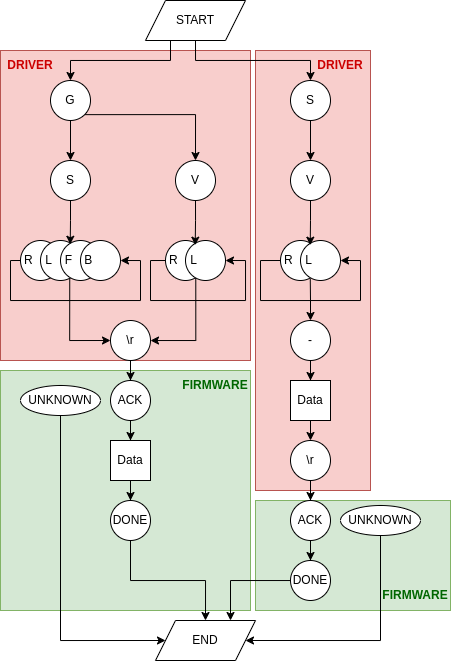
\includegraphics[width=100mm, keepaspectratio]{figures/ch3/protocol.png}
  \caption{A kommunikációs protokol}
  \label{fig:protocol}
\end{figure}

Tekintsük át a lehetséges üzeneteket. A firmware feladatainak defíniálásakor
tisztázódott, hogy kétfajta üzenet létezik, SET vagy GET, amely valamilyen
adatot mint érték kér, vagy vezérlő üzenet és a firmware valamely paraméterét
állítja. Ezeket az üzenetben rendre `s' vagy `g' karakter jelöli.

A mikrokontroller szenzorokkal távolságot mér, illetve enkóderek segítségével a
motorok sebességét. Ezáltal GET utasítás sebességre, és távolságra adható, ezeket
az üzenetben VELOCITY `v', illetve SENSOR `s' karakter jelöli. A továbbiakban
target-ként hivatkozom rájuk. SET parancs
értelemszerűen csak sebességre adható, így SET parancsot csak VELOCITY target
követhet: ``sv''.

A parancsot ezek után SENSOR target esetén maximum négy, VELOCITY target esetén
maximum két iránymeghatározó karakter követi. Ezek a FORWARD, BACKWARD, LEFT,
RIGHT irányhatározó rendre a `f', `b', `l', `r' karakterekkel. VELOCITY target
esetén csak LEFT és RIGHT irányhatározó karakter érvényes, lévén a robot két
motorral rendelkezik. 

GET parancs esetén az üzenetet carriage-return karakterrel zárhatjuk, és a
specifikált sorrendben várhatjuk a mikrovezérlő válaszát. Amennyiben SET
parancsot adtunk, úgy egy `-' karakterrel jelezzük a firmware számára hogy adat
következik. A küldendő adatot hexadecimális formában ASCII karakterekre kódolva
abban a sorrendben küldjük el, amely sorrendet az irányhatározó karaktereinkel
meghatároztunk. A megfelelő mennyiségű adat elküldése után a mikrovezérlő
nyugtázza a megkapott utasítást (ACK), majd annak végrehajtásáról DONE üzenetben
tájékoztat minket.

GET parancs esetén a firmware ugyanilyen formátumban biztosítja számunkra az
adatot. Az UNKNOWN, DONE és ACK üzenetek karaktereit rendre a `u', `n' és `k'
karakterek jelölik.

\medskip

\subsection{Szenzorok inicializálása és lekérdezése}

A firmwarenek feladata a szenzorok inicializálása. A mikrokontroller egy I2C
perifériát használ a szenzorok kezeléséhez, viszont mindegyik szenzorhoz
egyesével tartozik egy GPIO, amelyel a szenzor bootolása vezérelhető. A szenzorok
adatlapjából kiolvasható, hogy boot után a 0x52 címen érhetőek el. A bootfolyamat
késleltetésével a firmware fel tudja paraméterezni külön-külön az összes
szenzort, így azok a futás alatt saját címmel rendelkezhetnek.

Az inicializáció után a firmware aszinkron módon gyűjt adatot a szenzoroktól
amelyeket parancsra elérhetővé kell tennie a Raspberry számára. Ezzel az
architektúrával elkerülhető, hogy feladatok véletlenszerű felhalmozódása
bottlenecket képezzen a rendszerben, viszont megfelelően gyakori leolvasás esetén
megközelítőleg ugyanolyan pontos működést kapunk.

\subsection{Motorok sebességének mérése}

A mikrovezérlő dedikált timer perifériákat tartalmaz amelyek külön funkcióval
rendelkeznek az inkrementális enkóderek jeleinek feldolgozásához. A timerek
megfelelő inicializációja után a firmware feladata kiolvasni a timerek cnt
regiszterének értékét, majd ezekből az értékekből a robot sebességét valamilyen
algoritmus segítségével kiszámolni.

A sebesség algoritmusa függ a felhasznált alkatrészek fizikai paraméterétől, mint
a kerék átmérője, a motorokon használt áttétel, az enkódertárcsák beosztása,
valamint, ha a differenciális elrendezésből egy sebességértéket szeretnénk
defíniálni, a kerekek egymástól vett távolsága.

A sebességmérés pontossága függ az enkóder felbontásától, a kerék aktuális
szögsebességétől, valamint a lekérdezés időbeli pontosságától is.

A sebesség mértékegysége előre meghatározandó paraméter amit a firmware számára
specifikálni kell. Ezt a mértékegységet a robot léptékeihez és a feladatához
mérten mm/s egységben állapítottam meg.

\subsection{Motorvezérlés}

A motorok sebességének beállítása szintén a firmware feladata. A sebesség
beállítás komplex feladat is lehet, amennyiben nagy pontosságra törekszünk.

A motorok sebességszabályozásért felelős algoritmus állhat egy egyszerű PWM
állításból de egy komplex PID szabályzóból és szabályzókörből is. Az algoritmus
komplexitásának felső korlátja, hogy egy iteráció futásideje bele kell, hogy
férjen a szabályzó task periódusidejébe, amit a floating point unit hiánya
nagyban meg tud nehezíteni bizonyos sebesség felett.

A firmware specifikációja során nem határoztam meg pontos követelményeket, és a
végső kialakításban nem szerepel PID szabályzás, de a kódbázisban implementálva
van egy szabályzó, ami alkalmas lehet további fejlesztésre.

\medskip

A motor vezérlésénél fontos kérdés, hogy mi történjen ha elveszik a kapcsolat a
magasabb szintű vezérléssel. Robotikai alkalmazásokban általános megoldás, hogy
ilyen esetben a robot megáll, hiszen a funkcionalitás jelentős része kiesett, így
a robot akár károkat is okozhat. A folyamatos kapcsolat igényét a firmware
fejlesztése során szem előtt tartottam.

\begin{figure}
  \centering 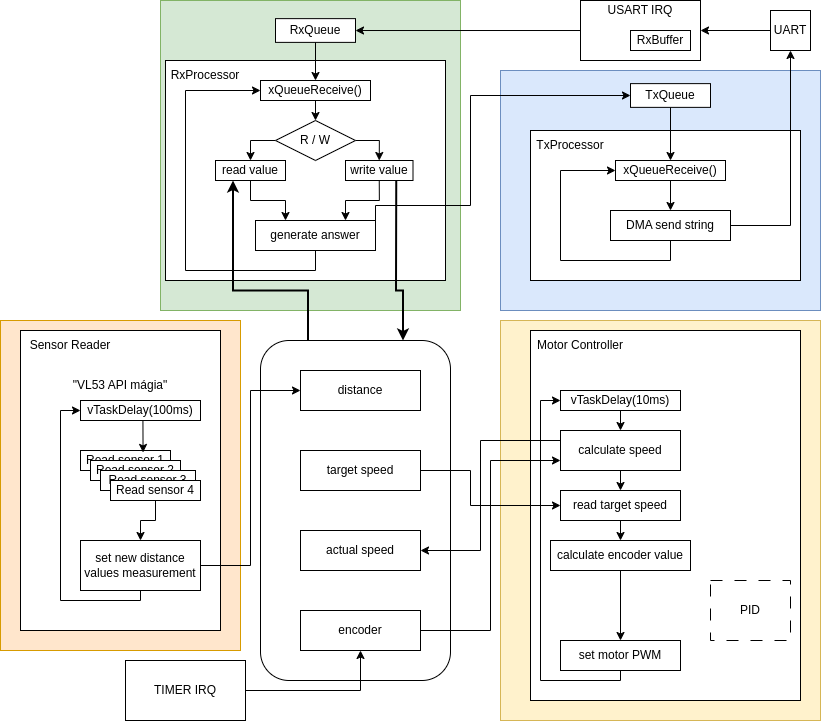
\includegraphics[width=150mm,
    keepaspectratio]{figures/ch3/firmware-architecture.png}
  \caption{A firmware blokkdiaggramja}
  \label{fig:firmware_arch}
\end{figure}

\section{Build}

A szoftverfejlesztés egy fontos eleme, hogy az adott build artifact könnyen
reprodukálható legyen. Az összetett fejlesztőkörnyezetek integrált toolchainjei
és komponensei ezeket a funkciókat általában megnehezítik, és megkötik a
fejlesztő kezét a felhasznáható eszközök terén.

A firmware fejlesztése alatt különleges figyelmet fordítottam rá, hogy munkám
széles körben elérhető eszközöket igényeljen csak a fordításhoz, és minél
modulárisabb, könnyebben cserélhető eszköztárra és projektkomponensekre bontottam
a feladatot.

A fordításhoz a GNU toolchain ARM mikrokontrollerek számára készült verzióját, az
\verb|arm-none-eabi-gcc|-t használtam. A többlépcsős build folyamat
végrehajtásához shellscriptekből és Makefileokból álló rendszert építettem, amely
a forráskódot viselkedés szerint modulokba engedi csomagolni, így többfajta
kialakítású projekt is könnyedén integrálható a buildbe. A nyelvi szerver
támogatáshoz \verb|clangd|-t használtam amihez a szükséges
\verb|compile_commands.json| file-t a \verb|bear| nevű, szintén open source
szoftverrel generáltam.

A projekt ezen felépítése lehetővé teszi hogy tetszőleges editorral (vim, emacs,
vscode) vagy fejlesztői környezettel megnyitható és szerkeszthető legyen.

A project teljesen verziókövetve van amihez git-et használtam. A repository
szabad licensz mellett elérhető a github linken\cite{RpirobotGitrepo}. 

\subsection{A project architektúrája}

A repository root könyvtárában két fontos mappát találunk, a \verb|utils| és
\verb|modules| mappákat. A \verb|utils| mappa tartalmazza a projekthez használt
általános scriptek legnagyobb részét. Ebben a mappában található scriptek a
következők:

\begin{itemize}
\item{build.sh:~A build folyamatot elindító script.}
\item{clean.sh:~A build artifactokat törlő script.}
\item{flash.sh~Az elkészült binárist ST-Linken keresztül a mikrokontrollerre
  másoló script.}
\item{openocd-start:~Az openocd service indító scriptje, amely on-chip
  debugoláshoz használandó.}
\item{openocd-start-bg:~Az openocd service indító scriptje, amely on-chip
  debugoláshoz használandó. A folyamatot háttérfolyamatként indítja.}
\item{gdb.sh:~Az arm gdb programot megfelelő indítási kapcsolókkal indító script,
  igényli az openocd futását.}
\item{gdb-ide.sh:~Az arm gdb programot megfelelő indítási kapcsolókkal a
  fejlesztőkörnyezetből indító script, igényli az openocd futását.}
\item{stm32f1x.cfg:~Az openocd által igényelt konfigurációs file a target
  mikrovezérlőhöz.}
\end{itemize}

A build egyszerűen végrehajtható a \verb|build.sh| script futatásával. A buildhez
tartozó konfigurációt a \verb|settings.sh| file tartalmazza, ami a repository
root könyvtárában található. A scriptben néhány hasznos beállítás amit
konfigurálni lehet:

\begin{itemize}
\item{A projekt neve}
\item{A fordító és linker binárisok}
\item{A kimenetet tartalmazó könyvtár}
\item{A fordításhoz és linkeléshez használt flagek}
\item{Az optimalizáció szintje}
\item{A lefordítandó modulok listája}
\end{itemize}

A projekt root könyvtárában található modules mappa további mappákat tartalmaz,
amelyek a projektben használt modulok.

A moduláris kialakításnak hála, egy új szoftverkomponens vagy library lefordítása
sokkal könnyebb és nem borítja meg a projekt addigi architektúráját. Egy modul a
modules mappán belül található olyan könyvtár amely tartalmaz \verb|module.sh|
scriptet.  A \verb|module.sh| script minden modulhoz meghatározza a fordítás
lépéseit, ami a leggyakrabban egy make parancs. A modul saját mappájában belül
dolgozik, és kimenetét egy obj nevű mappában gyűjti össze. A modul lefordulása
után ezek a kimenetek a modul nevének prefixálásával bemásolásra kerülnek a
projekt \verb|build| mappáján belül található \verb|obj| mappába. Ezzel a megoldással
elkerülhetjük, hogy két modul által ugyanazon a néven hívott object file
felülírja egymást.

A modulok jellemzően tartalmaznak egy \verb|Makefile|-t is, ami a pontos build
instrukciókat és a függőségeket is tartalmazza.

A modulok lefordítása és kimeneteik globális build mappába történő másolását
követően a build script meghívja a \verb|Make|-et a project root könyvtárából, ami a
linkelést elvégzi. Az így kapott kimenet egy ``.elf'' file, amely mellé
automatikusan generálódik egy ``.bin'' kiterjesztésű file, ami alkalmas a
mikrokontrollerre történő másolásra.

\medskip

A build folyamat végeztével az ST-Linket csatlakoztatva a fejlesztői
számítógéphez, a \verb|utils/flash.sh| scriptet futtatva a program letölthető a
mikrovezérlőre. 

\section{Felhasznált libraryk és keretrendszerek}

A firmware fejlesztéséhez több könyvtárat és eszközt használtam a projekt
áttekinthetősége, és a fejlesztés sebessége végett. A következőkben röviden
bemutatom a projektben használt librarykat és keretrendszereket. Röviden
bemutatom lényegi működésüket, indoklom szükségességüket a projekt szempontjából,
és kitérek előnyeikre és esetleges nehézségeikre is.

\subsection{FreeRTOS}

A firmware-ek felhasználási területükből kifolyólag gyakran real time
működésűek. Egy real time működésű program garanciát vállal, hogy meghatározott
időn belül biztosan választ ad. A real time működés elérését gyakran
nehezíti, hogy egy mikrovezérlő programja több feladatkört lát el egyidőben. Az
ilyen típusú multitasking környezetek megsegítésére real time
operációsrendszereket alkalmazunk.

Egy real time operációsrendszer nem garantálja a szoftver real time működését,
viszont lehetővé teszi, hogy real time működésű szoftvert fejlesszünk. Az
operációsrendszer eközben eszközkészletet biztosít a fejlesztő számára
a multitasking megkönnyítésére és a versenyhelyzetek, és IPC\footnote{IPC:~Inter
Process Communication} igények kezelésére. A firmware feladatainak
számából adódóan szükségesnek láttam egy operációsrendszer használatát.

Mikrokontrolleres alkalmazások tekintetében a legelterjedtebb beágyazott
operációsrendszer a FreeRTOS, amely egy ingyenes, nyílt forráskódú RTOS, 32 bites
mikrokontrollerekre lett tervezve.

A FreeRTOS operációsrendszer számos hasznos eszközt biztosít:

\begin{itemize}
\item{Konfigurálható kernel, többfajta ütemező algoritmussal.}
\item{Mutexek és szemaforok, szinkronizáció, és versenyhelyzetek kezelése
  céljából.}
\item{Opcionális dinamikus memóriakezelés, malloc, és free implementációkkal.}
\item{Taskok, Task prioritások, Taskkezelő mechanizmusok, függvények.}
\item{Message Queue-k, Notificationok, IPC megoldások.}
\end{itemize}

A firmware első modulja (a main modult leszámítva) a FreeRTOS
modul. Ez a projekt forráskód szinten elérhető, és rendkívül jól
dokumentált. A FreeRTOS monolitikus kialakítású, az operációs rendszer
egybe fordul a projektel. A main függvényben a
\verb|vTaskStartScheduler()| függvényhívással indíthatjuk el az
ütemezőt. Amely ezután ütemezi az előzőleg létrehozott taskokat.

Az operációsrendszer funkcióihoz API hívásokon keresztül férünk hozzá,
ezek vagy függvények vagy makrók formájában állnak rendelkezésre. A
FreeRTOS beállításait egy FreeRTOSConfig.h nevű headerben találjuk,
ehhez a filehoz referencia implementációt a FreeRTOS honlapján a
dokumentációban találhatunk. Fejlesztés előtt érdemes a rendszerrel
megismerkedni, és a használni kívánt rendszerhívások dokumentációját
átolvasni, erre a FreeRTOS honlapján az API
reference\cite{FreertosApiReference} szolgál.

\subsection{CMSIS}

Az ARM minden gyártótól aki ARM licenszelt architektúrát implementál
megköveteli, hogy termékük mellé készítsenek CMSIS támogatást. A
CMSIS, azaz Cortex Microcontroller Software Interface Standard, egy
szabvány amely az eszközhöz regiszterdefiníciókat és alapszintű
működéshez tartozó függvényeket biztosít. Segítségével elkerülhető,
hogy a fejlesztést megelőzően minden regiszterhez saját definíciót
kelljen készítenie a fejlesztőnek, vagy a driver kódban mágikus
konstansokat használjon regisztereléréshez.\cite{cmsis}

\medskip

A CMSIS a hardverhez legközelebbi szint, ahol olvasható kódot lehet C nyelven
írni. Érdemes megemlíteni, hogy csak CMSIS felhasználásával és egyéb absztrakciós
rétegek nélkülözésével rendkívül optimális kód írható. Erre a szintű
optimalizálásra azonban csak nagyon ritkán van igény, mert az adott feladathoz
használt mikrovezérlő rendszerint jelentős erőforrástartalékkal rendelkezik, így
a fejlesztést könnyítendő nincs szükség mikrooptimalizálásra. A CMSIS egyik nagy ereje,
hogy az absztrakciós library-k számára biztosít platformot. A másik fontos
alkalmazása, hogy a kód adott szegmenseiben lokálisan CMSIS kód alkalmazásával
biztosítja a mikrooptimalizálás lehetőségét a fejlesztő számára.

\medskip

A projekt keretein belül limitált mennyiségben használtam direkt CMSIS kódot,
lévén nem merült fel komoly igény ilyen mértékű mikrooptimalizálásra. Az aktuális
firmware fejlesztését megelőzően azonban volt kísérletem CMSIS alapú kód
fejlesztésére, amelyet a fejlesztés sebessége miatt nem tartottam ideálisnak,
ezért azt a projektet elvetettem, és új alapokra helyeztem a robot firmware
kódját.

\subsection{HAL}

Az STMicroelectronics biztosít két absztrakciós réteget a mikrovezérlőihez, ezek
az LL driver, valamint a HAL\footnote{HAL:~Hardware Abstraction Layer} driver. A HAL
driver egy magas szintű hardver absztrakciós könyvtár, amely minden STM32
perifériához tartalmaz driver réteget. A HAL kód könnyebben olvasható mint egy
CMSIS ellenben teljesítményében lassabb, és számottevően nagyobb méretű kódra
fordul.

A projekt fejlesztése során a HAL drivereket és saját kiegészítő kódot használtam
a mikrovezérlő hardvereivel történő interakcióban, ennek három fő indoka volt.

\begin{itemize}
\item{A HAL Driverek jól dokumentáltak, sok segédanyag érhető el velük
  kapcsolatban}
\item{Az STMicroelectronics CubeMX eszköze a HAL kód generálását támogatja.}
\item{A HAL Driverek felahsználásával lényegesen gyorsabban tudtam működő kódot
  létrehozni.}
\end{itemize}

Az STMicroelectronics biztosít egy fejlesztés segítő eszközt, az STMCubeMX
kódgeneráló és lábkiosztás menedzser programot. Ez a program integrálva elérhető
a CubeIDE fejlesztői környezetben, illetve standalone verziója is beszerezhető a
gyártó honlapjáról. A HAL driverek mellett szóló erős érv, hogy a projekt
inicializációja során a CubeMX által generált inicializáló kód nagyban
megkönnyítette a projekt bootstrapelését.

\medskip

A HAL driverek felhasználásának akadnak azonban hátrányai is. Ipari
alkalmazásában bizonyos feladatok megkövetelik, a HAL Driverek adott funkcióinak
helyettesítését. Erre a fejlesztés során közvetlen példát találtam.  USART stream
olvasása során a robot esetében számolni kellett azzal, hogy billentyűzetről
történő olvasással ellentétben a stream karakterei között nem lesz üres idő, és
egy karakter megérkezése után a következő karakter fogadása már folyamatban
van. Egy ilyen stream fogadását DMA vagy interrupt rutinok segítségével lehet
megvalósítani, ahol viszont az interrupt rutinnak megfelelően rövid idő alatt
kell lefutnia.

Pusztán HAL driverek felhasználásával ez nem lehetséges, mert az interruptos
olvasás újboli bekapcsolása a driverben reseteli az USART perifériát, amely így a
következő karaktert frame errorral fogja olvasni.

\subsection{VL53L1 API}

A VL53L1 szenzor egy teljes mikrovezérlőt magában foglaló távolságmérő eszköz,
meghajtása jelentősen eltér az I2C interfésszel rendelkező szenzorok döntő
többségétől. A projektbe történő integrálás során ez többször jelentett nagyobb
megakadást is.

\medskip

A VL53L1 szenzor, rengeteg belső funkcióval és konfigurációs lehetőséggel
rendelkezik, vezérlése komplex feladat. Az STMicroelectronics erre a problémára
válaszul kiadott egy forráskód szinten elérhető driver csomagot, amely
lefordítható tetszőleges architektúrára, és a szenzor vezérlését végzi.

A projekt során a szenzorok illesztésének feladata lényegétben ennek a drivernek
a beágyazása és lefordítása volt.  A driver több mint 30 forrásfile-ból áll, a
csomagban található dokumentáció valamint rövid readme, amely a driver
felhasználását hivatott bemutatni. A csomag implementál minden fontos vezérlő
logikát amely a szenzor vezérléséhez szükséges, ezekhez pedig publikus API
tartozik, amely függvények dokumentálva vannak a driverhez mellékelt API
dokumentációban. A driverben az I2C interfész kezelésére szolgáló függvények
nincsenek implementálva, ezek csak szimbólum szinten jelennek meg. Az integrálás
legfontosabb része ezeknek a függvényeknek az implementálása, amely a driver
számára lehetővé teszi az I2C interfész használatát.

Ez a feladat jelentős nehézségeket okozott, mert nem találtam pontos
dokumentációt az implementálandó függvényekről, azok helyéről, valamint a driver
beüzemeléséről, pusztán a teljes driver használatáról.

További nehézséget jelentett, hogy a driver több verzióban is megtalálható, és
több szenzorverzióhoz készült kiadás is elérhető, a driver csomagok között pedig
tévesen időnként Microsoft Windows operációsrendszerhez szánt teszt- és
kliensprogram is előfordult.

\medskip

Alapos kutatómunkát követően végül egy STMicroelectronics fórumbejegyzésben
találtam egy verziót, amely az ULD, azaz UltraLite Driver csomag nevet
viselte. Ennek a driver csomagnak hatalmas előnye, hogy csak a legszükségesebb
forráskódokat tartalmazza, és egyértelműen defíniálva van, hogy melyik függvények
implementálását igényli.

Ez a driver verzió azért jött létre, hogy a szenzorral ismerkedő fejlesztők vagy
fejlesztőcsapatok egy könnyebben áttekinthető projekt kereteiben használhassák az
eszközt. Ennek a kiadásnak további hatalmas előnye volt a projekt szempontjából,
hogy egy nagyságrendel kisebb a lefordított kód mérete, amely így a mikrovezérlő
flash memóriájában könnyedén elfér, a firmware egyéb részei mellett.

Az UltraLite Driver lefordításában és implementációjában nagy segítségemre volt
az ULD csomagban mellékelt példa projekt. A példaprojekt kódjából kiindulva
implementáltam az I2C periféria illesztését, és sikeresen teszteltem a szenzort.

\section{A firmware architektúra}

Az előző szegmensben bemutattam a felhasznált rétegeket, drivereket, és
könyvárakat. Ebben a részben bemutatom a firmware taskfelosztását, azok
architektúráját. Bemutatom a taskok kommunikációját, valamint a robot belső
memóriamodelljét, ami a robot paramétereinek firmware-en belüli modellje. 

\subsection{A robot belső állapota}

A firmware egy singleton adatstruktúrában tárolja azokat a paramétereket amik a
robot aktuális állapotát jellemzik. A robot ilyenmódon történő modellezése egy
helyen összesíti az összes paramétert így kiegészítés során elég ezt az egyetlen
struktúrát bővíteni.

A robot paramétereinek alstruktúrákba rendeződésével, modulok szerint
tagváltozókba csoportosítható minden fontos paraméter. A kód ezért olvashatóbb és
könnyen követhető, valamint lehetőséget ad a hosszú és nem beszédes változónevek
elkerülésére. Az alstruktúrák tartalmazzák a kérdéses adatokat valamilyen
formában, valamint többségük tartalmaz mutexet, amelyet a versenyhelyzetek
elkerülésére használ a firmware.

A struktúra négy fő alstruktúrából áll:
\begin{itemize}
\item{\verb|distance|:~A szenzorok által mért adat, négy darab előjel nélküli 16
  bites egész, valamint egy mutex.}
\item{\verb|encoder|:~Az enkóderpár jelenlegi, és előző iteráció beli értékei
  előjeles 16 bites egész formában.}
\item{\verb|actual_speed|:~A robot mért sebessége ami az enkóder értékekből
  számolódik, egy pár előjeles 16 bites egész, és egy mutex.}
\item{\verb|target_speed|:~A robot célsebessége, ami egy pár előjeles 16 bites
  egész, valamint egy mutex, és egy timeout 16bites előjel nélküli egész.}
\end{itemize}

A firmware elkülöníti a mért és kívánt sebességeket. A struktúra tagjai
közül három érhető el írásra és-vagy olvasásra, a firmware számára specifikált
utasítások szerint.

\medskip

A fent bemutatott struktúrán négy task, és egy interrupt rutin végez író- vagy
olvasó műveleteket. Rendszerint egy feladat a működését befolyásoló paramétereket
a struktúrából veszi, kimenetét a struktúrába írja vissza. A kövekezőkben
bemutatom a taskokat amelyek a robot funkcionalitását adják.

\subsection{Rx Task}

A firmware az USART felől érkező utasításokat egy külön taskban dolgozza fel. Az
üzenetek fogadásához azonban egy megszakításkezelő függvényt is felhasználok.

Az USART streamen érkező utasítások karakterenként érkeznek meg a vezérlőbe,
fogadásukat interrupt rutin végzi. Egy üzenet az első karakterétől (azaz az
utolsó stop bit után számíott első start bittől) számítva a carriage-return
karakter érkezéséíg tart. Az interrupt rutin feladata, hogy minden megérkezett
karaktert egy ideiglenes bufferben tárol, majd az első ``\textbackslash{}r'' karakter
megérkezését követően az üzenetet a parancsokat feldolgozó task számára egy
message queue-ba rakja. 

A periféria 115200 baud szimbólumsebességre lett konfigurálva, ez az interrupt
rutin számára felső korlátot jelent a futásidőre nézve, hiszen az interrupt
rutinnak a következő karakter megérkezése előtt be kell fejeznie futását. Az
olvasás egy gyors művelet, ellenben a message queueban való műveletvégzés egy
rendszerhívás ami az interrupt rutin kontextusában hosszú időt vesz igénybe.

A rutin futását nehéz utasítások számából kiszámítani ezért mérést végeztem. Az
interrupt handler első sorában egy GPIO lábat 1-es állapotba állítottam,
visszatérés előtt közvetlenül pedig reseteltem, így oszcilloszkóppal az impulzus
hossszából következtettem a rutin futásidejére.

\begin{figure}
  \centering 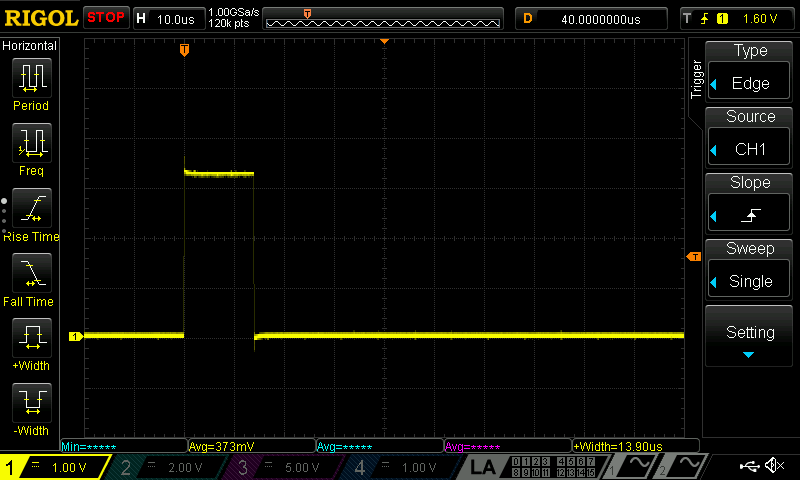
\includegraphics[width=150mm,
    keepaspectratio]{figures/ch3/osc_single_char_debug.png}
  \caption{Egyetlen karakter feldolgozásához szükséges idő debug módban}
  \label{fig:char_debug}
\end{figure}
\begin{figure}
  \centering 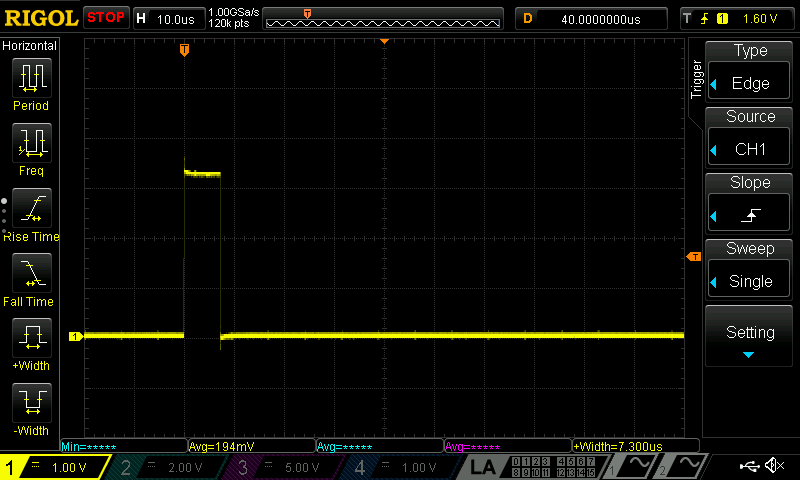
\includegraphics[width=150mm,
    keepaspectratio]{figures/ch3/osc_single_char_release.png}
  \caption{Egyetlen karakter feldolgozásához szükséges idő release módban}
  \label{fig:char_release}
\end{figure}
\begin{figure}
  \centering 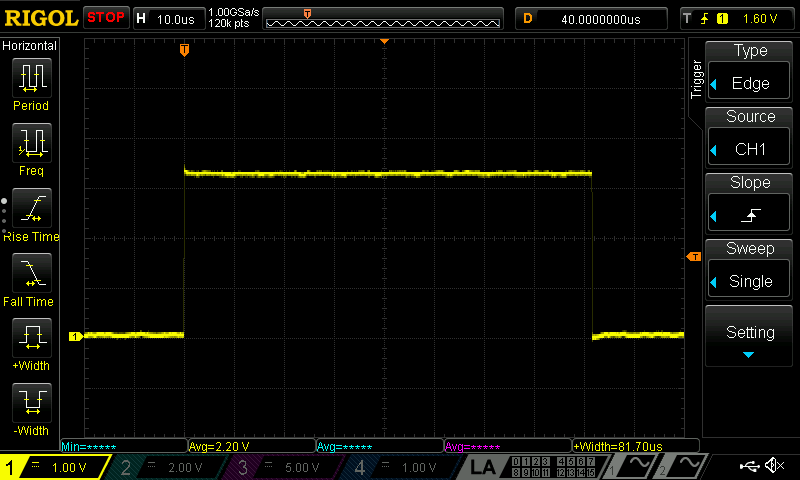
\includegraphics[width=150mm,
    keepaspectratio]{figures/ch3/osc_complete_message_debug.png}
  \caption{A kész üzenet fogadásának ideje az interrupt rutinban debug módban}
  \label{fig:msg_debug}
\end{figure}
\begin{figure}
  \centering 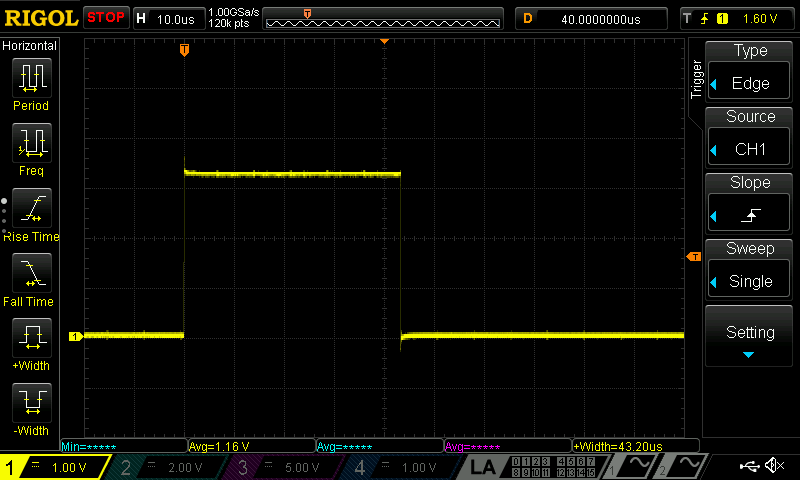
\includegraphics[width=150mm,
    keepaspectratio]{figures/ch3/osc_complete_message_release.png}
  \caption{A kész üzenet fogadásának ideje az interrupt rutinban release módban}
  \label{fig:msg_release}
\end{figure}

Az érkező karakterstream feldolgozásához szükséges feltétel, hogy a karaktereket
nagyobb sebességgel tudjuk fogadni, mint ahogyan azok megérkeznek. A szükséges
idő limitet a következő módon határoztam meg:

\medskip

Az USART konfiguráció 8N1 kialakítású, 115200 baud következésképpen az időkeret:

\begin{eqnarray*}
N_{karakter} = 10 \\
baudrate = 115200 \frac{1}{s} \\
T_{karakter} = N_{karakter} * \frac{1}{baudrate} s \approx 8.680555 * 10^{-5} s \\
T_{karakter} > 8.6 * 10^{-5} \\
\end{eqnarray*}

A fenti módszer segítségével meghatározható, a karakter-stream olvasásához
használt intterupt rutin futási idejére egy felső korlát, ezt $8.6 * 10^{-5}s$
-ban határoztam meg. A méréshez a kódot release és debug módban is lefordítottam,
az időkorlátoknak mindkét kód megfelelt. Az optimalizáció hatása látványos,
a~\ref{fig:char_debug},~\ref{fig:char_release},~\ref{fig:msg_debug},~\ref{fig:msg_release}
ábrákon jól megfigyelhető. Az interrupt rutin debug módban fordítva is 82 us
alatt fut le az üzenet endline karakterének fogadása esetében. Ez worst case
eset, amely a megállapított 86 us időnél kisebb. A kód release módban történő
futása esetén a tartalék sokkal nagyobb. 

\medskip
\textsl{
Érdekesség: A kód gyorsabb végrehajtása érdekében kísérletet tettem a függvény
flash memória helyett RAM-ból történő végrehajtására. Ennek a kísérletnek az
eredménye képpen a függvénynek az flashből történő végrehajtáshoz viszonyítva
több volt a futásideje. Ennek a jelenségnek az oka a végrehajtó architektúrájában
keresendő, a RAM ugyanis a harward architektúrának megfelelően nem a
kód végrehajtásra lett tervezve, így az utasítások felolvasása lassabb, még ha a
RAM sebessége elméletben a flash sebességénél nagyobb. Komplexebb
mikrovezérlőkben, amelyek nagyobb órajelfrekvencián működnek, ilyen esetekre egy
kis méretű utasítás-úti RAM modul is megtalálható, ahova a nagy sebességben
végrehajtandó kód betöltésre kerül.
}

\medskip

Fontos kiemelni, hogy a karakter stream időkorlátjának teljesítése nem elégséges
feltétele a helyes futásnak, a rendszernek ugyanis időre van szüksége a parancsok
értelmezéséhez és végrehajtásához is. Ennek érdekében egy message queue-t
alkalmaztam, amely egy FreeRTOS funkció. A message queue eltárol maximum 5
stringet, amelyeket a parancsfeldolgozó task kiolvas, és végrehajt. A queue
feltöltését az interrupt handler rutin végzi minden fogadott `\textbackslash{}r'
karakternél. A queue hatására rövid ideig tartó message burst-öt a firmware képes
lekezelni, és az üzenetekre érkezési sorrendben reagálni. 

\medskip

A parancsokat értelmező task az inicializációs fázist követően várakozik a
message queue-ba érkzező üzenetekre, amennyiben üzenet érkezik, úgy azt
végrehajtja. A parancsok a specifikációnak megfelelően értelmeződnek. Külön
függvényben történik a beérkező parancs értelmezése és bírálása, hogy
értelmezhető vagy ismeretlen utasítás. Értelmes utasítás hatására egy parancs
struktúra generálódik. A parancs állapotáról a task visszajelzést küld, ennek
végrehajhatósága esetén a generált parancs struktúrát egy végrehajtó függvény
kezeli, amely az állapotot módosító függvények meghívását végzi. 

\subsection{Tx Task}

A fogadást végző feladattól külön választva, egy sokkal egyszerűbb kialakítású
task kezeli az üzenetek küldését. Programszervezés szempontjából logikusabbnak
láttam, ha a küldés és fogadás külön taskokon keresztül történik.

A task felépítésében hasonlít fogadást végző társára, az elküldendő üzenetek egy
szeparált message queue-ba érkeznek, amelyből a task érkezés sorrendjében kiveszi
majd elküldi az üzeneteket.

Az üzenetek küldését a processzoridővel való takarékoskodás jegyében DMA
felhasználásával végeztem, így a task futásideje alacsonyan tartható. 

\medskip

A taskok inicializációjának sorrendjében megfigyelhető függőség, például az
RxTask nem válaszolhat, amig a küldést végző task nem fejezte be inicializációs
lépéseit. Ennek a befolyásolására a taskok létrehozásának sorrendje alkalmas
megoldás. Ez a megközelítés azonban olyan megoldáshoz vezet, ami a forráskódból
nehezen olvasható logikát implikál, a firmware esetleges átstruktúrálására a
rendszer érzékennyé válik.

Alternatív megoldásként a taskok inicializációs lépéseit kiegészítettem
szemaforok felhasználásával, amelyek segítségével a függő taskok blokkolnak,
ameddig függőségeik nem teljesülnek. Ennek a kialakításnak kis mértékben nagyobb
memóriaigénye van, lévén a taskokat szinkronizáló szemaforoknak szükséges
memóriaterület, de robosztusabb megoldás ami látványosabb is a kód olvasása
közben.

\subsection{Motor Task}

A motor vezérléséért felelős tasknak két fő feladatot kell ellátnia. A motor
sebességének vezérléséhez a PWM kitöltési tényezőt ki kell számítania, illetve a
motorok sebességét is ki kell kalkulálnia.

\subsubsection{Sebességmérés}

A sebesség pontos méréséhez egy timer periféria megszakítását használtam, lévén
az enkóder timerek perifériáinak olvasását minél pontosabban, azonos időközönként
kell olvasni. A megszakításkezelő rutin egy egyszerű feladatot végez, minden
meghívás alkalmával a robot paramétereit tároló globális struktúra enkóder
mezőjét frissíti. Mindkét motorhoz tartozó enkóder timer CNT  regiszterét
kiolvassa, majd az eltárolt előző értéknek beállítja az eltárolt jelenlegi
értéket, ezt követően a számlálóból kiolvasott értékkel frissíti a jelenlegi
számlálóértéket. A megszakítás kezelő értelemszerűen mindkét motor sebességét a
fenti módon frissíti. A rutin semmilyen többletfeladatot nem végez, mert az
időkritikus pont az új mérési eredmény pontos időben történő megszerzése, a
számítások elvégzésére a motorvezérlő task tökéletesen alkalmas.

\medskip

A motorok vezérlésének első lépése a sebesség meghatározása. Ezt az imént
bemutatott módon, az interrupt által kiolvasott enkóder értékekből végzi a
firmware. Az interrupt rutin csak kiolvassa a sebességet, azonban a task szintén
a rutin által írt memóriaterületet olvassa ami versenyhelyzetet eredményez. Arra
az időre, amig a task kiolvassa a robot paraméterei közül az enkóder értékeit,
kritikus szakaszt határoztam meg. Ennek a megközelítésnek nagy előnye, hogy nem
igényel mutex létrehozást, ami az időzítést tovább nehezítené, ellenben a
kritikus szakasz olyan rövid, hogy nincs lényegi ráhatással a rendszer többi
komponensének idejére. A kritikus szakaszban töltött idő alatt beérkező
megszakítások a szakaszból történő kilépéssel érvényre jutnak, így nem 
maradhat ki megszakítás sem.

A sebesség meghatározását ezek után egy egyszerű matematikai képlet segítségéve a
task már könnyedén elvégzi, a kiolvasott enkóderértékek, a kerék és motor fizikai
paraméterei és a megszakítás periódusideje alapján:

\begin{eqnarray*}
CNT = \text{az enkóder értéke} \\
N_{inkremens} = 14 \\
D_{kerék} = 21 mm \\
C_{kerék} = D * \pi \\
G_{áttétel} = \frac{1}{100} \\
t = 10 ms \\
s = \frac{C_{kerék} * CNT}{N_{inkremens} * G_{áttétel}} \\
v = \frac{s}{t} \\
\end{eqnarray*}

Tehát a kerék kerülete az átmérőből adódik, az enkóder egy teljes körülfordulás
alatt 14 lépést végez, a motor áttétele pedig egy tényleges körülfordulást 100
motortengely fordulással ér el. A CNT értékével skálázva megkapjuk a kerék által
megtett utat, amit a mintavétel periódusidejével leosztva megkapjuk a
sebességet.

A sebesség mértékegységének a mm/s mértéket választottam, amely a robot
feladatához  és méretéhez viszonyítva alkalmas méretarányban reprezentálja a
motorok sebességét.

A motor, áttétel, vagy kerék cseréje esetén a paraméterek újbóli megadása
szükséges, ezt a jelenlegi firmware verzióban egy header file-ban lehet
konfigurálni. 

\subsubsection{Sebességszabályozás}

A motor sebességének szabályozására az eredeti tervekben PI, vagy PID szabályzó
szerepelt. A firmware végleges megvalósításában a szabályzás megvalósítására már
nem maradt idő, ellenben a kód szerkezetének kialakításában figyeltem rá, hogy a
szabályzás könnyen integrálható legyen.

A projektnek része egy szabályzó algoritmus, amelyet külső könyvtár
részeként\todo{hivatkozás} integráltam a projektbe, a kód viszont nem került
végrehajtásra.

\todo{leírjam a szabályzás menetét, szabályzóhangolást?}
\todo{szabályozáshoz irodalomhivatkozás, jegyzet?}

A motor sebességszabályozása jelenleg a beállított sebességérték mint PWM jelet
vezérlő jellemző kerül direkt beírásra a timer ARR\footnote{ARR:~AutoReload Register}
regiszterébe. Ez a kialakítás a vezérlő logika számára lehetővé teszi a pontos
PWM beállítást, ellenben a hardverhez túlságosan közeli hozzáférést biztosít, ami
nem elegáns megoldás, lévén a firmware feladatai között szerepel a hardver
absztrahálása.

\subsection{Sensor Task}

Végül de nem utolsó sorban a firmware tartalmaz egy szenzor vezérlő taskot. Ennek
a tasknak a feladata a VL53L1 szenzorok inicializálása, egyedi címek kiosztása,
valamint a szenzorok periodikus olvasása, az UltraLite driveren keresztül.

\medskip

A task kezdeti lépésben négy címet hoz létre, amivel a szenzorokat
inicializálja. Az inicializáció során a szenzorokat a hozzájuk rendelt GPIO
lábakon keresztül egyesével, egymás után bootolja be, majd egyedi címmel látja el
őket. A már bebootolt szenzorok csak a nekik kiosztott egyedi I2C címekre fognak
válaszolni, így a soron következő eszközt alapértelmezett gyári címén megszólítva
az inicializáció elvégezhető. A sensorok helyes működéséről és állapotukról
visszajelzést adnak, amit polling jellegű megoldással, driver támogatással
vizsgál a task.

Az összes szenzor bebootolását követően a task fő ciklusában egyesével
végigolvassa a szenzorokat, amelyek, amennyiben van elérhető mérési adat, azt
visszaküldik a vezérlő fele. A szenzorolvasó task ezt követően a robot
paramétereinek struktúrájába, a megfelelő alstruktúrába beírja az értékeket. A
struktúra mutexel védett, lévén a szenzorolvasó taskal párhuzamosan a
parancsvégrehajtásért felelős task olvashatja a mért távolságértékeket. 

\section{Értékelés, Fejlesztési lehetőségek}

A firmware fejlesztése összetett feladat volt, a fejlesztés során sok új
tapasztalatra tettem szert.

\medskip

Az elkészült verzió komponensei jó összhangban működnek egymással, az időzítési
feladatokat is megfelelően sikerült kivitelezni. A felhasznált hardver elégséges
volt a feladathoz, bár adott alkalmakkor a feladatot könnyítette volna egy
nagyobb teljesítményű mikrovezérlő alkalmazása.

A projekt során átható és mély ismeretekre tettem szert a fordítás, és a build
folyamatok tekintetében, az elkészült projektstruktúrát egyéb projektek
esetében is hasznosnak ítélem.  

A projekt moduláris kialakítása nagy segítség volt a fejlesztés alatt, a rendszer
átláltható, és karbantartható maradt, a javítások és kiegészítések rendszerint
könnyen megvalósíthatóak voltak.

\medskip

A projekt ezek ellenére számos hiányosságot, és fejlesztési lehetőséget is
tartalmaz. 

A robot nagy hiányossága, hogy a motorok szabályozása nincs implementálva. A
szabályzás implementálásához a motorokon rendszeridentifikációt kell végezni,
majd az így kapott rendszerhez PID szabályzót hangolni. A paraméterek kiszámolása
után a firmware részét képező szabályzót a mért értékekkel kell inicializálni, és
a motorvezérlésben a szabályzó iterációs függvényét meg kell hívni.

\medskip

A robot kommunikációján szintén van fejlesztési lehetőség. A kommunikáció jelen
állapotában nehezen tolerálja a hibákat, egy hibatűrőbb kommunikációs protokoll
kifejlesztésével, amely hiba esetén esetleg újra építi a kapcsolatot,
robosztusabb megoldás lenne elérhető. 

\medskip

A firmware két kisebb fejlesztési lehetőséget tartalmaz, amelyeket érdemes
megemlíteni.

Alacsony sebességeken a sebességmérés nem ad pontos eredményt, a
sebesség csökkenésével alternatív megoldásra való áttérés esetén ez javítható.

A robot sebességét a hardver konfiguráció befolyásolja, azonban a
firmwareben a konfiguráció csak újrafordítás során lehetséges. A robot
paramétereit tároló struktúra elemeiként defíniált hardveres
konfigurációval ez a limitáció megszűnhet, amely konfigurációt akár a
Linux file-rendszerben rendszerben is tárolni lehetne.


%% %----------------------------------------------------------------------------
\chapter{A Linux rendszer}
%----------------------------------------------------------------------------

Az előző fejezetek során bemutatásra került a robot mechanikus modellje,
moduljai, azok feladata, célja, és megvalósítása. Részletesen elemeztem a
firmware fejlesztését, feladatát és kialakítását is. Ebben a feladatban a robot
központi vezérlésére használt Raspberry Pi mikroszámítógépen futó
operációsrendszer és szoftveres környezet felépítéséről és kialakításáról írok
bővebben.

\medskip

A robot magasabb szintű vezérlése erőforrásigényes feladat, kialakításához egy
nagy teljesítményű processzoros rendszerre van szükség.  A nagyobb számítási
kapacitású rendszerekhez és szoftveres megoldásokhoz azonban összetettebb
operációs rendszerre van szükség, ami az erőforrások menedzselését hatékonyan
tudja végezni, és biztosít egy olyan platformot amin a rendszer kezelése, és
magas szintű nyelven írt programok futtatása ergonómikus és hatékony környezetben
tehető meg.

Beágyazott környezetben a leggyakrabban előforduló magas szintű operációsrendszer
a Linux. Ezt a népszerűséget többek között ingyenes, open source modelljének,
lelkes közösségének és flexibilis, kis erőforrásigényű kialakításának köszönheti.
A GNU/Linux mérnöki körökben elterjedt választás asztali felhasználásban is. A
Linux kifejezés önmagában csak a kernelre utal, az operációsrendszer magjára,
amely a feladatütemezésért, és taskmanagementért felel. Egy teljes rendszer
magában foglalja a GNU/Linux kernelt, shell és init programot, és egyéb, a
feladat által meghatározott szükséges könyvtárat, scriptet és binárist. A teljes
rendszercsomagot, amely egy feladatot teljeskörűen ellátni képes disztribúciónak
nevezzük.

\medskip

A Linux rendszer open source kialakításából következik, hogy a célplatformra
(megfelelő támogatás megléte mellett) forráskódból lefordítható. A fordítás
feladata azonban nem triviális feladat, amely manuálisan nagy erőfeszítéseket
igényel, valamint nagy hibakockázattal jár. A feladat mértékét csak növeli, hogy
minden a célplatformon használni kívánt szoftvert és könyvtárat szintén le kell
fordítani és a rendszerrel együtt csomagolni. A disztribúciókészítés fáradtságos
feladatát buildrendszerek alkalmazásával igyekszünk könnyíteni. Ezek a rendszerek
általánosságában a folyamatot scriptek segítségével automatizálják amely két
fontos előnnyel jár. Egyfelől a disztribúciókészítés a script vagy scriptek
konfigurálásával könnyen befolyásolhatóvá, a build folyamat pedig
reprodukálhatóvá válik. Másfelől elosztott fejlesztést tesz lehetővé, az egyes
komponensekhez tartozó build scripteket külön fejlesztők vagy fejlesztőcsoportok
tarthatják karban, így a fordítószkriptek és csomagok karbantartása elosztott
feladattá válik amely egy közösségen (ideális esetben) egyenletesen el tud
oszlani. 

\medskip

A fejezet első részében bemutatom az operációsrendszer működését, és
komponenseit. Kifejtem a bootolás folyamatát, szükséges programokat és
konfigurációkat. Röviden összefoglalom a rendszerben szükségszerű programok
funkcióját, feladatát és felhasználását.

A fejezet második részében a disztribúció elkészítéséhez használt eszköz, a
Yocto Project működését mutatom be.

A fejezet harmadik és utolsó részében a saját disztribúció tervezését,
kialakítását, fejtem ki. Specifikálom az előállítandó rendszer tulajdonságait és
feladatát. Bemutatom a saját csomagjaimhoz tartozó build
scripteket, és patcheket, és az egyes feladatok eléréséhez végrehajtott
konfigurációs lépéseket. Végeredményben értékelem a kész disztribúciót, és
javaslatokat teszek annak fejlesztésére.

%% \section{A Linux}

%% A Linux napjaink legelterjedtebb iparban használt operációsrendszere,
%% megtalálhatjuk minden nagyobb teljesítményt igénylő informatikai eszközünkben. A
%% routerek és networkswitchek szinte kizárólagosan Linux rendszert futtatnak, de
%% megjelenik kisebb beágyazott eszközöktől elkezdve a szervereken keresztül egészen
%% a szuperszámítógépekig egyaránt.

%% A mobiltelefonok platformján legnépszerűbb operációsrendszer, az Android szintén
%% is Linux alapú. Napjainkban az asztali felhasználása is egyre inkább teret nyer
%% köszönhetően a személyre szabhatóságának, teljesítményének és ingyenességének.

%% \subsection{Eredete}

%% A Linux egy Unix-like operációs rendszer. Eredetileg egy Minix klónként indult
%% amelyet Linus Torvalds Finn származású informatikus kezdett el fejleszteni, hobbi
%% projekt szintjén. A rendszer iránt hatalmas volt a lelkesedés, így 1992-es első
%% kiadásától napjainkig aktív fejlesztés alatt áll. 

%% \medskip

%% A fejlesztésben a Linux projekt körül kialakuló közösség aktívan részt vesz. A
%% projekt népszerűségének egyik nagy oka a nyílt forráskód, amelyet bárki igénye
%% szerint elolvashat, és módosíthat saját felhasználási céljainak megfelelően. A
%% projekt jelenleg a GPLv2 licensz alatt érhető el.\todo{kernel.org hivatkozás}

%% A Linux azonban nem pusztán egy közösségi kezdeményezés amely lelkes fejlesztők
%% hobbiprojektje. Fejlesztésében számos nagyvállalat aktívan vállal szerepet. Az
%% infrastruktúrában betöltött központi szerepe miatt kontribúciók érkeznek számos
%% chipgyártó vállalattól, akik saját termékeik támogatottságát szeretnék
%% biztosítani a Linux kernelben, de a felhőalapú szolgáltatásokat biztosító tech
%% óriások is rendszeresen támogatják a projektet.

%% A Linux az eddig valaha volt legnagyobb szoftveres projekt, amelyen a legtöbb
%% fejlesztő dolgozott. A fejlesztés ilyettén módja az ipar minden résztvevőjének
%% kölcsönösen előnyös, az elosztott fejlesztés pedig széleskörű hibakeresést, és új
%% funkciók gyors implementálását teszi lehetővé.

\section{Az operációs rendszer felépítése}

Egy Linux alapú operációs rendszer több részegységből áll, ezek egymást
elfedő rétegekként, vagy egymásra épülő szintenként képzelhetőek el. A Linux,
pontosabban szólva GNU/Linux önmagában csak a kernelt foglalja magában, egy
teljes rendszer működéséhez azonban több egyéb komponensre is szükség van.

Egy ilyen komponens például egy extra kernel modul, amely a kernel
funkcionalitását hivatott kibővíteni, például valamilyen hardver támogatásának
biztosításával, vagy egy init program ami a rendszer bootolása során elsőként
indított program és a szolgáltatások elindításáért felelős. A rendszer szerves
részei továbbá a file-rendszer, interaktív felhasználás esetén shell, és
szövegszerkesztő, alapvető parancssori alkalmazások (coreutils). Természetesen
extrém esetekben a szerkesztő, parancssori alkalmazások, vagy akár shell nélkül
is futtatható Linux kernel, és általa ütemezett szolgáltatások, azonban a
felhasználási esetek döntő többségében ezeknek a megléte nagyban megkönnyíti,
sőt, lényegében lehetővé teszi a rendszer karbantartását és a hibakeresést, ezért
szinte sosem maradnak ki egy disztribúcióból.

\subsection{Kernel}
 
A kernel feladata, hogy a rendelkezésre álló erőforrásokat elossza a
végrehajtandó feladatok között, valamint platformot adjon ezen feladatok közötti
kommunikációnak. Absztrakciós rétegként működik, amely a futtató hardver és
perifériák, valamint a felhasználói programok között teremt kapcsolatot. A kernel
megléte két szegmensre bontja a Linux rendszert, kernelspace és userspace
szintekre.

\subsubsection{Kernelspace és userspace}

A kernelspace minden olyan kódot futtató egységre értendő, amely a
kernel privilégium szintjén fut, és általában közvetlen interakcióban áll
hardverrel. A kernelspace kód rendkívül érzékeny terület, mert bármilyen hiba a
rendszer teljes összeomlásához vezethet, ezért a kernel módosítása, fejlesztése
komplex feladat, amely hatalmas szakértelmet igényel. A kernelspace kódban ezért
csak a feltétlenül szükséges dolgok vannak implementálva, mint például az
ütemező, az IPC és task szinkronizációs megoldások, valamint a hardver
meghajtásához szükséges driver modulok. 

A userspace tartalmaz minden egyéb komponenst. A userspace fejlesztés rendszerint
sokkal könnyebb feladat, mert az esetleges hibák nem vezetnek a rendszer teljes
összeomlásához így a hibakeresés sokkal könnyebb feladat. A kernel által a
userspace alkalmazások számára biztosított funkciókat az alkalmazások
úgynevezett rendszerhívásokon keresztül érhetik el. Rendszerhívás esetén a
program megszakítja futását, és átadja a vezérlést a kernelnek. A kernel elvégzi
a kért feladatot, majd a vezérlés visszatér a userspace alkalmazáshoz.

\subsubsection{Scheduler}

A kernel alapja egy ütemező, angolul scheduler. Ennek a komponensnek a feladata,
hogy a számítási teljesítményt és a processzor időt elossza a futtatandó taskok
között. Az ütemező a kernel egyik legfontosabb komponense, működésének módja
meghatározza az operációsrendszer teljesítményét adott feladatok elvégzésében.

\medskip

A kernel az ütemezőn keresztül minden task számára saját virtuális processzort és
stacket biztosít. Ez a gyakorlatban azt jelenti, hogy a program futása közben nem
észlel változást az ütemezésből kifolyólag, mer minden kontextusváltás esetén az
aktuális kontextus elmentődik, és az új kontextus kerül betöltése. A változások
azonban a rendszer többi komponensében végbemehetnek, így ha a program a rendszer
többi részével lép interakcióba, az esetleges versenyhelyzetet okozhat. A
versenyhelyzetek feloldására, és a taskok közötti hatékony kommunkikációra a
kernel többféle megoldást is kínál. 

Ilyen eszközök a message queue-k, a shared memory, amelyek üzenetküldésre és
kommunikációra használható eszközök, valamint a mutexek és szemaforok, amelyek a
versenyhelyzet kezelésére, valamint a taskok szinkronizálására alkalmasak.

\subsubsection{Modularitás}

A Linux kernel eredetileg monolitikus kernel, azaz egy lefordított oszthatatlan
program, amelynek módosításához az egész kernel újrafordítására van szükség. Ez a
kialakítás sok szempontból nem optimális hiszen minden új eszköz csatlakoztatása
esetén az eszközhöz tartozó drivert bele kell fordítani a kernelbe, valamint ha
probléma lép fel a kernel egy részében, az az egész rendszert destabilizáljal.

Az említett első probléma áthidalása érdekében a fejlesztés során több módosítást
végeztek a Linux kernelen, és egy moduláris kernelt hoztak létre, amely támogatja
a különböző modulok dinamikus betöltését, és ezáltal a kernel funkcióinak runtime
alatt történő kiegészítését. A modulok betöltésének megvalósításához dinamikus
linkelésre volt szükség. A dinamikus linkelés azt jelenti, hogy a program futás
közben, külső file tartalmát képes saját magához linkelni, a betöltést követően
linkelt modulban megvalósított funkcionalités már elérhető a kernelből.

A modulok egyik nagy felhasználási területe a különböző eszközökhöz használt
driverek dinamikus kezelése. A kernel forrás módosítása nélkül egy modul
lefejlesztésével elérhető, hogy egy hardver támogatva legyen a kernel által.

A modularitás azonban nem oldotta meg a monolitikus kernelek nagy hátulütőjét,
mégpedig a rendszer stabilitását. A monolitikus kialakítás miatt ha instabil
modulok kerülnek betöltésre az az egész kernel számára fatális következményekkel
járhat. Egy rosszul működő modul könnyedén az egész rendszert tönkreteheti, ezért
új modul betöltésénél fokozott elővigyázatosságra van szükség. Szerencsére a
kernel, és a modulokat kezelő alkalmazások fel vannak készítve a modulok egyszeri
betöltésére. Egyszeri betöltés esetén amennyiben a betöltött modul hibát okoz,
akkor a rendszert újraindítva a kernel a modul betöltése nélkül indul így a hiba
esetén a fejlesztésre használt rendszer nem válik használhatatlanná.

\subsection{Init}

A kernel önmagában nem végez célfeladatot, csak a feladatot ellátó programoknak
biztosít platformot. A Linux rendszerben a feladatokat service-ek, azaz háttérben
párhuzamosan futó alkalmazások és alkalmazáscsoportok végzik. Az alkalmazások
futásukban erősen függenek egymástól, ebből a függőségi gráfból pedig fa
rajzolható. A bootfolyamat során a megfelelő service-ek automatikus elindításáért
az init program felel.

\medskip

Az init program egy kitüntetett program, amelyet a kernel argumentumként kap meg,
és elsőként indít el. Egy Linux rendszerben a programok elindítása mindig egy
szülő programból indított ``fork\(\)'' és esetlegesen azt követő ``exec\(\)''
rendszerhívásokkal érhető el, így minden folyamatnak létezik szülőfolyamata. A
fenti szabály alól egyedül az init program kivétel, ennek a programnak a
feladata, hogy konfigurációs scriptek felhasználásával a bootolás során a
szükséges rendszerfolyamatokat megfelelő sorrendben elindítsa.

Több implementációja is ismert, legismertebb és legelterjedtebb verziója a
systemd, amely az asztali célra szánt disztribúciók döntő többségében
megtalálható. Beágyazott alkalmazások esetében gyakran előfordul ezen felül a
SysVinit, ami egy régebbi egyszerűbb init implementáció, szűkebb
funkcionalitással. Ennek ellenére beágyazott környezetben gyakran elegendő
funkcionalitást nyújt.

Az init programokhoz rendszerint scriptek megírásával tudunk bootkonfigurációt
létrehozni. Egy konfigurációban meghatározott sorrendben indulnak el a defíniált
folyamatok. A bootolást követően az init program feladata a háttérben futó
programok, szakkifejezéssel daemonok kezelése, amelyhez az init program
parancssori frontendet biztosít. Így lehetőségünk van a rendszer szolgáltatásait
futásidőben is konfigurálni.

\subsection{Shell}

A legtöbb rendszerben kritikus, hogy legyen valamilyen felhasználói bemenet,
amelyet Unix-like rendszerek esetében általában egy shell program biztosít. A
shell egy szöveges parancsértelmező alkalmazás, általános célja, hogy a
renszerhez egy kezelőfelületet biztosítson. A shell rendszerint a rendszerrel
való interaktív kapcsolatbalépés alapvető eszköze. Parancsai alapvető programok,
amelyek a disztribúció részét képezik, és általában a \verb|coreutils| nevű
package részei. Ezekkel a programokkal alapvető file-műveletek és minimális
rendszerkarbantartás végezhető.

A shell programok rendszerint biztosítanak scriptelési lehetőséget is. A
shellscriptek a rendszer alapvető elemei, felhasználásukra számtalan helyen
találhatunk példát. Bonyolultabb programok, vagy programcsoportok elindítására,
vagy ismétlődő feladatok automatizálására shellscript készítése bevett és
praktikus megoldás.

Különböző shell implementációk léteznek, beágyazott környezetben a leggyakrabban
a bash, és dash shellekkel találkozhatunk. Asztali környezetben számos egyéb
shell típus létezik, például zsh, ksh, és a fish.

\subsection{GUI}

A shell interfészen kívül a Linux operációs rendszerek képesek grafikus
felhasználói felületet is biztosítani. Grafikus felületre beágyazott környezetben
nem minden esetben van igény, az esetek jelentős részében a feladat ellátására
egy shell teljesen megfelelő. Akadnak azonban feladatok, ahol a grafikus
megjelenítés része a feladatkörnek, vagy a rendszer karbantartásában jelenthet
segítséget egy grafikus környezet.

\medskip

A Linux rendszereken grafikus megjelenítésre két fő protokollt, az X11 és Wayland
protokollokat szokás alkalmazni.

A két megoldás közül az X11 (vagy röviden csak X) a régebbi rendszer, fejlesztése
napjainkban nagyon lassan halad. Gyakran fogalmazódik meg kritika az elavúlt
technológia miatt, ennek ellenére az X a gyakrabban használt megoldás.
Kialakítása szerver-kliens kapcsolat alapú.  A program elfedi a ki és bemeneti
perifériákat, mint egér billentyűzet és monitor, és ezek eléréséhez interfészt
biztosít az alkalmazások számára.  Kialakításának jellegzetessére a régi
számítástechnikai rendszerek maradványa, amely szerint egy központi számítógéphez
több végpont csatlakozik, a megjelenítést a végpontok végzik, míg a
számításigényes feladat a központi rendszeren fut. Ez a megközelítés napjainkban
kevésbé praktikus, a számítógépek elterjedésének köszönhetően.

A wayland egy modernebb, korszerűbb protokol és architektúra, amely a grafikus
alkalmazások megjelenítésére lett kifejlesztve. Koncepcióját tekintve egyszerűbb
és kisebb az erőforrásigénye. Központi komponense egy úgynevezett wayland
compositor, amelyet minden grafikus környezet saját maga implementálhat. A
wayland biztosít egy nyelvet amin keresztül ezzel a compositor-ral
kommunikálhatnak alkalmazásaink.

\section{A boot folyamat}

A kisebb komplexitású, mikrokontrollereken használt operációs rendszerekkel
ellentétben egy Linux alapú rendszer boot folyamata komplexebb, és több időt is
vesz igénybe. A boot folyamatot fázisokra bonthatjuk, amelyek időben egymást
követik, és mindegyik fázis az időben utána következőt készíti elő, egészen a
teljes rendszer felállásáig.

\subsection{BIOS}

A bekapcsolást követően az alaplapba égetett firmware azaz a
BIOS\footnote{BIOS:~Basic Input Output System} indul el. Ennek a rövid programnak
a feladata a POST azaz Power On Self Test öntesztelő eljárás végrehajtása, majd a
megfelelő bootloader betöltése az MBR szerint. Az MBR azaz Master Boot Record az
első szektorban található kis terület amely tartalmazza a bootloader
információit, valamint a partíciós táblát. Ezek alapján a BIOS elindítja a
megfelelő bootloadert.

\subsection{Bootloader}

A bootloader egy kicsi és kompakt program ami az operációs rendszer komplex
indítását hivatott elősegíteni. Képes akár több kernel imaget is kezelni, és fő
feladata a kernel image betöltése a memóriába. Asztali környezetben, X86
architektúrán leggyakrabban a GRUB2\footnote{GRUB:~Grand Unified BootLoader} nevű
bootloaderrel találkozhatunk. A programot rendszerint csak GRUB-nak nevezik,
lévén teljesen leváltotta az első verziót.

Beágyazott környezetben gyakran az U-Boot\footnote{U-Boot:~Universal Boot}
szolgál a kernel betöltésére. Az U-Boot egy teljesértékű bootloader, amely a
teljes bootfolyamatért felel, ellentétben a GRUB-bal, amely csak úgynevezett
``second stage'' bootloader. U-Boot ARM architektúrájú rendszereken jellemző.

\subsection{Kernel}

A bootloader által betöltött program az operációsrendszer magja, a
kernel. Betöltés után egy bootoláshoz használt előre tömörített speciális
fájlrendszert, az initramfs-t betölti a memóriába ami biztosítja a kernel számára
a megfelelő eszközöket a rendszer elindításához. A következő lépésben a kernel
további hardver inicializációkat hajt végre majd felcsatolja a root
fájlrendszert. Végül utolsó lépésben elindítja az init programot amelyel a
bootolás a userspace-ben folytatódik.

\subsection{Init}

Az init program a processek között egyedülálló módon a 0 process id-val
rendelkezik, és gyökérpontja a processtree-nek. Az init program ezt követően az
init scriptekben meghatározott módon elindítja a rendszerfolyamatokat, és a
rendszer megkezdi működését.

\section{Build}

A Linux operációs rendszer egyik legnagyobb előnye, hogy az egész rendszer
forráskódjához szabad hozzáférésünk van, módosítható és fordítható. Fordítása
azonban összetett és bonyolult feladat, amelynek automatizálására több
keretrendszer is épült. Ezek a keretrendszerek általában megkönnyítik a fordítás
folyamatát, konfigurációs interfészt biztosítanak a kernelhez, illetve adnak
olyan eszközöket, amelyek segítségével a végső image könnyedén elkészíthető. Az
iparban két fontos rendszer terjedt el: a Buildroot, valamint a Yocto Project.

\medskip

A Buildroot egy Makefile és patch gyűjtemény amely segít a forráskód
lefordításában, valamint a root fájrendszer generálásában. A konfigurációban
többek között a menuconfig, és kconfig TUI\footnote{TUI:~Terminal User Interface}
programok biztosítanak felhasználóbarát felületet. 

Általános vélekedés szerint a Buildroot könnyebben tanulható, egyszerűbb
konstrukció. A build rendszer Makefile alapú, ami széles körben ismert a
fejlesztői körökben, így egyszerű módosítások elvégzése könnyebb feladat lehet. A
Buildroothoz azonban sokkal kevesebb cég biztosít supportot, a projektet
jellemzően a közösség tartja karban.

\medskip

A Yocto Project egy umbrella project, amely az openembedded build systemet, és
hozzá tartozó általános receptcsomagokat foglalja össze, és biztosít egy
referencia disztribúciót, amelyet poky-nak nevez. A projekt konfigurációja
scripteken keresztül történik, amely szkriptek használnak Python és shellscript
részleteket, valamint az openembedded build engine, a bitbake saját script
szintaxisában megírt scripteket.

A projekt első számú nagy előnye a széleskörű támogatottság. A Buildroottal
ellentétben a legtöbb gyártó biztosít Yocto támogatást saját termékeihez. A
projektet a Linux Foundation is támogatja, ezek fényében a projekt aktívan és
dinamikusan fejlődik. 

A rendszer sajátossága a buldscriptek, a Yocto terminológia szerint receptek,
rétegekbe szervezése, amely így átlátható rendszerbe foglalja ezeket. A
kialakítás rendkívül flexibillisé teszi a konfigurációt.

A build során a projekt shared state chache-t használ, amelynek köszönhetően a
build folyamat az első build alkalmával lassú, (lassabb mint a Buildroot)
ellenben a további buildek, esetleges konfigurációk módosítása esetén már sokkal
gyorsabban futnak le, így a hibajavítások, és új funkciók implementálása által
igényelt idő sokkal kevesebb, mert nem kell minden változtatás után az egész
fordítást újra elvégezni.  

A projekt hátránya, hogy a kialakításából adódóan sok időt vesz igénybe amíg a
fejlesztő megérti és átlátja a build folyamatot. A konfigurációhoz használt
szintaxis szintén új megtanulandó elem, így a projekt tanulási görbéje
kivételesen meredeknek mondható.

\medskip

A projekt során nagyobb komplexitása ellenére a Yocto projectet választottam,
amely szabadabb fejlesztést és személyre szabhatóságot tesz lehetővé.

\subsection{A Yocto Project felépítése és működése}

A Yocto project komplex és robosztus build rendszer, működésének megértése
kritikus a hatékony munkavégzéshez. A projekt egyik nagy előnye az átfogó és
részletes dokumentáció, amelyet a Yocto honlapján\todo{hivatkozás és source}
találunk. A dokumentáció részletes utasításokat ad számunkra a kezdeti
lépésekhez, amelyet követve az első teszt build könnyen megvalósítható.

A project saját terminológiát használ aminek megértése a működés megértését
nagyban segíti. A következő szegmentsben bemutatom a projekt felépítését, és
leggyakrabban használt kifejezéseinek jelentését.

\subsubsection{Bitbake}

A Yocto Project központi komponense a Bitbake build eszköz, amely az openembedded
projekt központi build eszköze is. A Bitbake végzi a csomagok előállítását a
beágyazott Linux rendszerhez.  A program egy úgynevezett ``task execution
engine'', amely feadatát scriptekben defíniált alfeladatokból való függőségi gráf
építésével, és ezek végrehajtásával végzi.

\medskip

A Bitbake saját script nyelvel rendelkezik, amely szintaxisában hasonlít a
bashscript és Python nyelvekhez. A hasonlóság odáig terjed, hogy a scriptek
magjában teljes Python vagy bash nyelvű függvények találhatóak. A Bitbake
scriptekre használt általános kifejezés a recept, a receptek pedig általánosan
``.bb'' kiterjesztéssel rendelkeznek.

A script legfontosabb feladata különböző taskok létrehozása, és a működésüket
befolyásoló változók értékének beállítása. A Bitbake ezen scriptekből határozza
meg az elvégzendő feladatok listáját, valamint a feladatok egymás közötti
függőségeit. 

\subsubsection{Recept}

A Bitbake számára végrehajtható script, a recept, amely segítségével csomagok
előállítását végezzük. Az openembedded rendszerben minden csomaghoz és
előállítandó komponenshez tartozik egy recept, amely az előállítás pontos
lépéseit tartalmazza. A meghatározott lépések szigorú sorrendben egymás után
hajtódnak végre:

\begin{itemize}
\item{do\_fetch}
\item{do\_unpack}
\item{do\_patch}
\item{do\_configure}
\item{do\_compile}
\item{do\_install}
\item{do\_package}
\end{itemize}

A fenti lista nem teljes, csak átfogó képet hivatott adni egy átlagos csomag
lefordításának lépéseiről. Első lépésben a forráskód letöltése történik, amelyen
kicsomagolás után patcheket alkalmazunk. Ezután a build konfigurációja,
következik, amit a forráskód lefordítása követ. A kész build artifacteket ezután
egy célkönyvtárba telepítjük, és csomagot készítünk belőlük. 

A Yocto renszerének nagy előnye, hogy a receptek módosíthatóak. A működés során
használt változók kiegészíthetőek, vagy éppen teljesen megváltoztathatóak, de a
végrehajtandó feladatokhoz is be tudunk szúrni kiegészítéseket. A
kiegészítésekre úgynevezett ``.bbappend'' fileok szolgálnak, amelyek a velük
azonos nevű recepthez tartalmaznak kiegészítéseket.

A receptek dinamikus módosíthatósága és kiegészíthetősége a Yocto Projectet
rendkívül flexibilissé teszi.

\medskip

A receptekhez tartozó másik fontos koncepció a gyakran használt kód külön fileban
tárolása, erre a célra a ``.bbclass'' fileok szolgálnak. A bbclass fileok olyan
scripteket, és kódokat tartalmaznak, amelyeket több receptben is újra kívánunk
használni, ezzel elkerülhetjük, hogy a gyakran ismételt kód másolásával, vagy
újra megírásával időt pazaroljunk.

\subsubsection{Layer}

A receptek csoportosítására a Yocto Project terminológiája szerint ``layer''-eket
használunk. A layerek nem mások, mint jól szervezett mapparendszerbe gyűjtött
receptek, amelyek tipikusan egy jól körülhatárolható funkcionalitást
biztosítanak. Ilyen funkcionalitás lehet egy adott feature támogatás, mint
például a Python könyezet, vagy valamilyen hardver támogatás
biztosítása. Ezutóbbi layereket BSP\footnote{BSP:~Board Support Package}
layereknek nevezzük. A build konfigurációban lehetőségünk van megadni a
layereket, amelyekből recepteket használni szeretnénk, valamint ezekhez
prioritások társításával sorrendet meghatározni.

A gyakorlatban a layerek git repositoryk, amelyeket a projekt root könyvtárába
klónozva érhetünk el. Tartalmaznak egy layer konfigurációs állományt, amelyben a
layerhez kapcsolódó információk és beállítások érhetőek el. A konfiguráción kívül
a layerekben mappákba szervezve megtalálhatunk konfigurációs fileokat,
recepteket, bbappend fileokat, és patcheket is. Egy réteget tartalmazó mappát
hagyományosan a ``meta-'' kifejezéssel kezdjük, és a biztosított funkcióval
zárjuk, például: ``meta-python'', a réteg amely Python funkcionalitást biztosító
recepteket tárol. 

A layerek egymásra rétegződése elegáns megoldás, amely jól szervezett elosztott
munkavégzést tesz lehetővé. A gyakorlatban egy projekt általában egy layerben
határozza meg a saját receptjeit, amely így könnyen verziókövethető is. A
layerben lehetőségünk van függőségek defíniálására, ezzel meghatározva a pontos
szükségleteket a saját buildkonfigurációnk számára. 

\subsubsection{Verziók és kiadások}

A Yocto Project egy dinamikusan fejlődő rendszer, amely mind saját működésében,
mind a biztosított package-k verziójában aktívan fejlődik. A dinamikus fejlődés
mellett a projektben kihívást jelent a függőségi gráf betartása a packagek
között, ezért a fejlődést rendszerint verziók kiadásával rendelik
mérföldkövekhez.

A kiadott verziók lehetnek LTS\footnote{LTS:~Long Term Release} vagy standard verziók,
amelyek a verzió támogatásának idejét határozzák meg. Minden layer karbantartó
külön branchen kezeli saját layerének azon verzióját, amely egy támogatott Yocto
release-hez tartozik, így a layerek klónozása után a használni kívánt Yocto
verziót a ``git checkout'' parancsal állíthatjuk be. A layer verziójának a hibák
elkerülésének érdekében meg kell egyezniük a használt Yocto verziójával.

\subsubsection{Poky}

A Yocto Project új projektek kezdéséhez egy referenciadisztribúciót biztosít
amely segítségével a projekt dinamikusan bootstrapelhető. Ez a disztribúció nem
keverendő a Linux rendszerek disztribúcióival, tisztán csak a build rendszer
csomagjáról van szó.

A biztosított referenciadisztribúció neve Poky, amely tartalmaz egy openembedded
rendszert, és kiegészítő layereket, amelyek a legtöbb alapvető és gyakran
használt funkcionalitást biztosítják.

\subsubsection{Build konfigurációk}

A build konfigurációt több összetevő határozza meg. A projekt gyökérkönyvtárában
találunk egy \verb|oe-init-build-env| nevű scriptet, amelyet
source-olva\footnote{Fontos hogy source-oljuk a scriptet, mert a buildfolyamathoz
használt környezetet ez a script állítja be shellünkben, ha futtatni próbáljuk
úgy hibát is jelez!} a projekthez szükséges környezet beállthatjuk, valamint
létrehozhatjuk a buildfolyamatok által használt mappát, ennek alapértelmezett
neve a \verb|build|.

A mappában találunk egy \verb|conf| mappát, amelyben a buildhez használt lokális
konfigurációk kapnak helyet különböző fileokban. Ilyen például \verb|local.conf|
file amelyben például a célarchitektúrát határozhatjuk meg, amelyre a
keresztfordítást végezzük. A mappában találjuk továbbá a \verb|bblayers.conf|
file-t amelyben a felhasznált layereket tudjuk specifikálni, amelyben a Bitbake a
recepteket keresheti.

\medskip

A kívánt eredmény, amelyet végsősoron elő kívánunk állítani, egy image file,
amelyen a teljes rendszer megtalálható. Ezt az image-et adathordozóra másolva,
egy bootolható médiát kapunk, amelyel a céleszköz megkezdheti működését. 

Egy image előállítását egyszerre befolyásolja a lokális konfiguráció, valamint a
receptek által meghatározott build konfiguráció, ezek összességében eredményezik
a rendszer kimenetét. 

\subsubsection{Kezelés}

A Yocto több eszközt is biztosít számunkra, amelyel a fejlesztés során felmerülő
feladatokat meg tudjuk oldani. Ezek a feladatok rendszerint kézzel is könnyedén
elvégezhetők, de a rendszer által biztosított parancsokkal általánosságában
könnyen tudjuk a projektet konfigurálni.

\medskip

A buildfolyamatot a Bitbake indításával kezdhetjük el. A program kapcsolók nélkül
indítva átvesz egy argumentumot, amely a végrehajtandó recept, majd a recept
alapján végrehajtja a szükséges feladatokat. A receptet a bitbake kiterjesztés
nélkül várja! A Bitbake-et egy recept végrehajtásához a következő módon
indíthatjuk el:

\begin{verbatim}
    $ bitbake <recept>
\end{verbatim}

A Bitbake a parancs hatására kezdeti lépésben beolvassa a \verb|bblayers.conf| és
\verb|local.conf| fileokat, majd az ezekben meghatározott módon beolvassa az
recepteket. A cél receptből kiindulva, a receptek tartalmazta feladatokból
függőségi fát épít, majd nekilát a feladatok végrehajtásának.

A build tesztelésére, esetlges konfigurációkra több kapcsolóval befolyásolhatjuk,
amelyek a bitbake felhasználása során nagy segítséget jelenthetnek, a teljesség
igénye nélkül néhány:

\begin{itemize}
\item{\verb|-e|:~A build során alkalmazott változókat listázza}
\item{\verb|-k|:~A build esetleges failelése esetén nem áll le, hanem minden
  feladatot végrehajt, amely nem függ a hibába futó feladattól}
\item{\verb|-c|:~A build során csak egy meghatározott feladatot hajt végre}
\end{itemize}

\section{Saját Linux image készítése}

A robot következő modulja a beágyazott Linux image, ennek elkészítéséhez a Yocto
Projectet használtam. Ebben a szegmensben a fejlesztés menetét fogom bemutatni.

\subsection{Specifikáció}

A Linux rendszer elkészítéséhez első lépésben specifikáltam az igényeket,
amelyeket ki kellett elégítenie az image-nek. Az igények felmérését követően
lehetséges megoldásokat kerestem, amelyeket kipróbáltam és teszteltem. A Linux
platform a robot esetében host platformként viselkedik, amely a ROS keretrendszer
futtatását végzi. A rendszernek azonban meg kell felelnie egyéb igényeknek is.

\subsubsection{Kapcsolat}

A rendszer vezeték nélkül vezérelhető legyen. Egy autonóm alkalmazásban a
legpraktikusabb megközelítés, ha a kommunikáció vezeték nélkül történik, a
robotban használt Raspberry Pi ehhez hardveres támogatást is biztosít. A
legideálisabb helyzetben a kapcsolat a fejlesztőeszközön és a roboton kívül nem
igényel egyéb támogatást, így ezt opcionális célnak tűztem ki.

\subsubsection{Soros port}

A rendszernek kommunikálnia kell tudni a vezérlőpanellel soros porton keresztül.
A kommunikációs csatorna kritikus, hiszen a ROS számára feltétlen szükséges, hogy
a hardverhez hozzáférjen, az ehhez defíniált protokol pedi USART kommunikációt
igényel.

\subsubsection{ROS}

A rendszernek futtatnia kell a ROS2 keretrendszert. A ROS2 rendszer
futtatása a legfontosabb feladat amely a linux rendszerre hárul. A
keretrendszeren kívül a saját ROS projektek futtatása szintén feladat, amelyek a
robot hardvert integrálják a ROS2 rendszerbe, valamint a magas szintű
funkcionalitást implementálják. A node-ok automatikus indítását nem tűztem ki
feladatul, mert úgy számoltam, hogy a rendszer idő hiányában nem fogja elérni a
teljes autonóm mozgást, így a ROS node-ok automatikus indítása kevésbé fontos
kritérium, valamint a parancssorból történő indítás implementációja után az
automatikus indítás egy triviális feladattá egyszerűsödik.

\subsubsection{Egyéb}

A könnyű feladatvégzés és tesztelés érdekében a rendszerbe egyéb packageket
telepítettem, mint szövegszerkesztő, file manager. Ezek a rendszernek nem
közvetlen részei, de meglétükkel a tesztelés és a rendszer használata sokkal
ergonómikusabb. 

\subsubsection{Build}

A buildel szembeni egyedüli igény, hogy minden fentebb specifikált funkciót és
konfigurációt generáljon bele az elkészített rendszer rootfilesystem-jébe. Így a
legkevesebb utómunka szükséges a deploymenthez, és a legjobban használató ki a
Yocto Project.

\subsection{Projekt layer: meta-rpirobot}

A feladat végrehajtását egy saját layer defíniálásával kezdtem, amelybe az image
generálásához szükséges receptek és fileok kerülnek. A layer alkalmas a munkám
verziókövetésére, valamint későbbi reprodukálására is. A fileok rendszerezése az
általános konvenciók szerinti felépítést követi. A layer tartalmaz egy conf
mappát, amelyben a layer.conf a layer beállításait tartalmazza.

A build szempontjából a legcélravezetőbbnek tartottam a Yocto Project legújabb
LTS kiadását, a kirkstone verzót használni. Ebből kifolyólag a saját layerem is a
kirkstone verzióval kompatibilis.

\subsubsection{Layerkonfiguráció}

A konfigurációban a layer tulajdonságait állíthatjuk be. Konfigurálható a
szükséges layerek listája, amik a layer függőségeiként szolgálnak, a kompatibilis
Yocto kiadás, valamint a receptek elrendezésének módja, ami alapján a bitbake
megtalálja a recepteket.

A layer függőségeit az alapvető layereken felül a meta-ros, meta-raspberrypi
és a meta-ros2-humble rétegekkel egészítettem ki.

A receptek és fileok megtalálásához konvenció szerinti alapértelmezett
beállításokat használtam. Ezek értelmében a recepteket a generált package nevével
ellátott mappa tartalmazza, amely mappákat általánosabb kategóriájuk szerint
recept-könyvtárakban tároljuk, az alábbi módon:

\dirtree{%
  .1 meta-rpirobot.
  .2 conf.
  .3 layer.conf.
  .2 LICENSE.MIT.
  .2 recipes-core.
  .3 busybox.
  .4 busybox.
  .5 udhcpd.conf.
  .4 busybox\_1.35.0.bbappend.
  .3 hostapd.
  .4 hostapd\_2.10.bbappend.
  .4 patch.
  .5 hostapd.conf.patch.
  .3 images.
  .4 rpirobot-core-image.bb.
  .3 init-ifupdown.
  .4 patch.
  .5 init-ifupdown\_1.0.bbappend.
  .3 ros-components.
  .4 files.
  .5 LICENSE.
  .4 ros-rpirobot-driver\_0.1.bb.
  .4 ros-rpirobot-interfaces\_0.1.bb.
  .3 wpa-supplicant.
  .4 wpa-supplicant.
  .5 wpa\_supplicant.conf-sane.patch.
}

Az ábrán látható, hogy a recipes-core mappában találhatóak a szükséges package-k
mappái, amelyeken belül a receptek és appendfileok találhatóak. 

\subsection{Az első boot}

A kész image előállítását egy Raspberry Pi-n bootolni képes image előállításával
kezdtem. A teljes image generálása komplex feladat, ennek megkönnyítésére a Yocto
Projectben egy \verb|core-image-minimal| recept is szerepel, amely leírása
alapján egy minimális Linux rendszer amely képes bootolni a target platformon. A
projektet tehát ennek az image-nek a generálásával kezdtem. A buildhez a
\verb|build/conf/bblayers.conf| fileban ki kellett egészíteni a layerlistát, a
Raspberry Pi támogatását biztosító meta-raspberrypi layerrel. Ezt követően a
\verb|build/conf/local.conf| fileban a machine változónak a ``raspberrypi4\-64''
értéket adva beállítottam a target platformot. Ezek után a core-image-minimal
targetet a Bitbake meghívásával előállítottam, majd bmaptools segítségével SD
kártyára másoltam az elkészült imaget. A bootolás tesztelvén a Raspberry Pi-hez
egy USB-USART átalalkító áramkörrek kapcsolódtam, majd megkíséreltem a bootolást,
amely sikeres volt.

\subsection{Image}

Az image generálást szintén receptek végzik, így a \verb|meta-rpirobot| layerben
a \verb|recipes-core/images| mappában létrehoztam egy receptet, ahol az image
elkészítéséhez szükséges feladatokat és konfigurációkat állíthatom be, ennek a
receptnek az \verb|rpirobot-core-image| nevet adtam.

A Bitbake támogatja a receptek további kiegészítését, ezért a legkézenfekvőbb
megoldás, a \verb|core-image-minimal| ``öröklése'' volt, ezt az inherit
kulcsszóval lehet megtenni.

A konfiguráció teszteléséhez licensz és summary beállításokat végeztem, majd az
image-et az említett hasznos eszközöket tartalmazó packagekkel egészítettem
ki. Ezek előnye hogy a Yocto alapértelmezett layereiben megtalálható a receptjük,
telepítésük pedig egyszerű, és minimális a hibalehetőség. Ezért a build
tesztelésére, és később az image-en való munka során is hasznos csomagok.

A telepített csomagok a vim, mc, bash, tmux, és a screen csomagok voltak. Egy
sikeres build lefuttatása után tapasztaltam, hogy az image az elvárt módon
tartalmazza ezeket a programokat. 

\medskip

A receptben az image kiegészítéséhez létezik egy alternatív mód, amely néhány
funkció esetében nagyban megkönnyíti a konfigurálást. Ez a funkció az image
feature amely lényegében teljes csomag- és konfigurációhalmazt jelent, amely az
image számára valamilyen teljes feature-t biztosít. A funkció az
\verb|IMAGE_FEATURES| változóhoz való hozzáfűzéssel érhető el, például a
következő képpen:

\begin{verbatim}
    IMAGE_FEATURES += "package-management"
\end{verbatim}

A fenti kóddal package managert, és a package managementhez szükséges egyéb
eszközöket telepítettem az image-re.

\subsection{A kapcsolat}

Az image fontos feladata, hogy vezeték nélküli kapcsolaton keresztül legyen
elérhető, ennek legkézenfekvőbb megoldását a beépített WiFi modul
felhasználásában láttam.

A kapcsolat kiépítésére WiFin keresztül két módon van lehetőség. Az egyik mód a
WiFi modult access point módban konfigurálni, amelyben a Raspberry Pi saját
hálózatot nyit, amelyhez bármilyen WiFi-képes eszközzel csatlakzhatunk. Az
autentikációra egy alapértelmezett és egyszerű jelszó generálható, amelyet az
első bejelentkezés után a felhasználó szabadon megváltoztathat. Ez a kialakítás
nagyon előnyös, mert nem igényel semmilyen külső eszközt, csak a fejlesztői
számítógépet valamint a robotot.

Alternatív megvalósításként a robot csatlakozhat egy előre bekonfigurált WiFi
hálózatra, amelyen innentől kezdve elérhető. Ez a megvalósítás sokkal egyszerűbb,
mint az access point kiépítése, ellenben a robot vezérléséhez valamilyen külső
eszköz és infrastruktúra megléte szükségeltetik, amelyet ráadásul a robot
konfigurációjának megfelelően kell beállítani. A megoldás további hátránya, hogy
a robotot helyhez köti, bár ez az állapot a robot feladatköréből adódóan nem
biztos, hogy tényleg problémát jelent, valamint könnyen orvosolható is, ha a
helyzet azt kívánja. 

\medskip

Első nekifutásra az access point konfigurációval próbálkoztam, a fent ismertetett
előnyei miatt. A konfigurációhoz hozzáadtam a hostapd csomagot, valamint a
\verb|busybox-udhcpd| csomagját. A hostapd az access point létrehozásáért és
üzemeltetéséért felelős szoftver, a \verb|busybox-udhcpd| pedig a busybox csomag
által szolgáltatott lightweight dhcp szerver, amely csatlakozó eszközök számára
szolgáltat ipcím kiosztást. A csomagok telepítése mellett appendfileokat hoztam
létre, amelyek a konfigurációt módosították a kívánt módon.

Több sikertelen tesztelési fázis, és hibakeresés után sikerült olyan
konfigurációt beállítanom, amelyben a robot saját hálózatát felállította, és a
csatlakozó eszközök számára ipcímet is szolgáltatott.

A kialakítás sajnálatos módon rendkívül instabil volt, gyakran fordult elő, hogy
a kapcsolat rövid időre megszakadt, amely használhatatlanná tette a megoldást. A
hibát minden valószínűség szerint a WiFi chip teljesítményének, vagy az
alkalmazott on-board antenna kialakításának nem megfelelősége okozta. A probléma
javítására külön WiFi eszköz beépítése egy praktikus megoldás, ilyen külső eszköz
amelyet USB-n keresztül lehet csatlakoztatni, könnyen be is szerezhető. A
fejlesztési idő miatt azonban tovább kellett lépnem és alternatív konfigurációt
kellett fejlesztenem.

\medskip

A végleges megoldásban a robot egy előre meglévő hálózathoz automatikusan
csatlakozik, ameyet a wpa-supplicant csomag konfigurációjával értem el. A külső
hálózatot egy telefonon indított hotspot hálózat biztosította. A hátrányokkal
együtt ez a kialakítás már sokkal stabilabban működött, így lehetőség volt tovább
lépni.

\medskip

\subsection{A layer index}

A felhasznált csomagok megtalálásában a leghasznosabb eszköz az
openembedded layer index volt. Ez az openembedded által jóváhagyott rétegeket
gyűjtő adatbázis, amelyhez egy webes frontend is tartozik. A weboldalon alkalmunk
nyílik layereket, és recepteket keresni, amelyekről az adatbázisból hasznos
információkat tudhatunk meg.

\todo{forrás}
A hálózati konfiguráció, valamint a telepített csomagok a meta-openembedded
layerben a meta-networking és a meta-oe alrétegekben voltak megtalálhatóak,
amelyeket ezért a layerlistához kellett adnom.

\subsection{Az USART port}

A soros kommunikáció a robottal kritikus feladat volt a ROS komponensek
telepítése és tesztelése előtt, lévén a saját komponensek a robot többi részével
UART interfészen keresztül tartják a kapcsolatot. Az USART port konfigurálását a
Raspberry Pi esetében azonban a bootfile-ok módosítását igényli.

A Raspberry Pi pinsorán kivezetet USART-on megjelenik egy konzol, amelyre
csatlakozva lehetőségünk nyílik az eszköz vezérlésére, egy teletype-on
keresztül. Ez a megoldás hasznos, ugyanis az eszközhöz kapcsolódhatunk akkor is
ha a hálózat meghibásodik, vagy egyéb okokból nem elérhető, ugyanakkor ennek a
portnak a felhasználásával könnyen csatlakoztatható a robot vezérlőpanelje is.  A
teletypeok menedzseléséért felelős service Linux rendszer alatt a \verb|getty|,
ennek konfigurációját azonban script állítja elő a build során, így
praktikusabbnak láttam a konfigurációt létrehozó scriptet befolyásoló változók
konfigurálását a végső script patchelésénél.

Az usart porton két jelenség történik, amelyet a port használatához el kell
kerülni. Az első,hogy a bootolás során a kernel üzenetei ezen a porton keresztül
jelennek meg, a másik, hogy a bootolást követően ezen a porton egy shellhez
csatlakoztatott teletype jelenik meg, amely ellehetetleníti a kommunikációt.

A fenti működéseket kikapcsolni a local.conf konfigurációba írt három sorral
lehet:

\begin{verbatim}
    ENABLE_UART = "1"
    SERIAL_CONSOLES = ""
    CMDLINE_SERIAL = ""
\end{verbatim}

Az első sor a build során inicializálja az USART-ot amelyen ezek után
kommunikálni lehet, majd a második és harmadik sor kikapcsolja az usarton
megjelenő parancssori interfészt, és kernelüzeneteket, így a port teljesen
szabadon marad a szükséges célra.

Fontos, hogy változók beállítása hatástalan, amennyiben azt az image-et generáló
receptben hajtjuk végre, ellenben a local.conf-ban történő beállítás sikerre
vezet. 

\subsection{A ROS keretrendszer}

A ROS2 keretrendszer integrálására a projekt hivatalos layerét használtam. A
layer a projekt fejlesztésével párhuzamosan fejlődött, így több frissítésre is
volt szükség mire a build sikeresen lezajlott.

A \verb|meta-ros| layer az openembedded kialakítás szerint egy repositoryban több
layert tárol, így a \verb|meta-ros| klónozása után a \verb|bblayers.conf| filet
több layerrel is kiegészítettem, ezek a \verb|meta-ros2|,
\verb|meta-ros2-humble|, \verb|meta-ros-common|. A ROS erőteljesen épít a Python
nyelvre, így függőségeinek kielégítéséhez a \verb|meta-openembedded| layer,
\verb|meta-python| sublayerét is felhasználtam.

A layerek kiegészítése után, a ROS telepítési útmutatóját követve az image
receptben meghatároztam a használni kívánt ROS disztribúciót, inicializáltam az
útmutató szerint a buildhez szükséges változókat, majd az ``IMAGE\_INSTALL''
változót bővítettem a ros-core, ros-base csomagokkal, valamint néhány example
kategóriájú csomaggal, amelyek a disztribúció tesztelésében nyújtottak
segítséget.

A build végül sikeresen lefutott, és az image flashelése után a Raspberry Pi-n
képes voltam a ROS beépített példamoduljait futtatni. 

\subsection{A saját ROS packagek}

A ROS projekt önmagában egy keretrendszer, a robot működéséhez a buildnek
automatikusan tartalmaznia kell a robothoz készült ROS packageket is. Ezeknek a
packageknek a fordításához a meta-ros layer többi receptjét vettem alapul,
valamint a ROS2 fórumokon más olyan projekteket, amelyek saját recept
lefordításán alapultak.\todo{source?}

A projekt során elkészített ROS package-ekről a következő fejezetben részletesen
lesz szó, a jelenlegi fejezetben csak lefordításuk és buildrendszerbe történő
integrálásukat tárgyalom.

A projekthez két ROS package készült el, amelyekhez a fordítást a ROS az ament
buildrendszer segítségével végezi el, amely CMake és Python alapú packagek
létrehozására szolgáló rendszer. A meta-ros layer az ament felhasználására
biztosít lehetőségeket, így a package-k integrálása kisebb erőfeszítések árán
megoldható: 


\begin{verbatim}
asdfsadfasfdas
\end{verbatim}
\todo{ide a fontos parancsot beírni, a csomagkészítéshez}

A két package közül egy \verb|ament_cmake|, egy pedig \verb|ament_python|
buildrendszert használ, ezekhez külön scriptek készültek a
\verb|recipes-core/ros-components| mappában.

A receptek felépítése mindkét esetben rendkívül hasonló. Elsősorban a recepthez
tartozó weboldalt, maintainert, valamint rövid leírást kell kitölteni, amit a
licensz file, és hozzá tartozó checksum követ.

A ros külön változókba gyűjti a fordításidejű és futásidejű függőségeket, ezek
megadása a következő feladat. 

A Yocto rendszerben minden forrás valamilyen upstreamről kerül letöltésre, a
packagek esetében ez a github repository, amelyen tároltam őket. Ennek az
upstreamnek a megadása a következő lépés, amely során nem csak az upstreamhez
tartozó URL-t, hanem a branch, és githash értékeit is meg kell adni a pontos
verzió letöltéséhez. 

\todo{valami formát találni a kódsoroknak}
A packagek fordításához tartozó feladatokat az inherit ros\_ament\_cmake, vagy
inherit \verb|ros_ament_python| sorokkal csatolhatjuk a recepthez, ami a továbbiakban
már tudni fogja hogy milyen lépéseket kell végrehajtani a ROS package
lefordításához.

Utolsó lépésben a csomaghoz tartozó \verb|FILES| változó értékét kell beállítani
olymódon, hogy kiegészítjük, minden csomagba telepítendő fileal, ami a receptek
esetén a következő sorral volt kivitelezhető:

\begin{verbatim}
    FILES:${PN} += "/usr/share/<csomagnév>/*"
\end{verbatim}

\subsection{Fejlesztési lehetőségek}

A build végeredményében egy sikeres és használható disztribúciót állít elő,
amelynek konfigurációját teljesen automatikusan végzi el. A saját réteg
alkalmazásának megfelelően a reprodukció könnyen és gyorsan végrehajtható, hiszen
ahhoz csak a layerek klónozására van szükség, amelyeket a kirkstone branchre
állítva a lokális konfiguráció kiegészítésével már indíthatjuk is a build
folyamatot. 

A rendszer ugyanakkor több fejlesztési lehetőséget is tartalmaz. A fejlesztés
során a hálózathoz csatlakozás mellett döntöttem a fejleszés sebessége és az
időkeret miatt. Egy új WiFi modul csatlakoztatásával és integrálásával az
instabilitás orvosolható lehet, és a robottal való kommunikáció egy elegánsabb
módon valósítható meg. 

A Raspberry Pi több USART portal is rendelkezik, az egyszerűség kedvéért a
projekt során a legkönnyebben elérhetőt választottam. A soros port meghagyása
azonban debuggolás szempontjából hasznos biztonsági tartalék. A konfiguráció
tovább fejleszthető olyan módon, hogy egy másik port kivezetésével az eredeti
megőrizhető erre a célra.

A ROS projekt ugyan integrálva van a buildben, ellendben automatikus indítása nem
megoldott. A rendszer egy setup script source-olását igényli, amely a
futtatókörnyezetet állítja be a ros számára. A rendszerben használt shell, a bash
inicializációs fileját kiegészítve ez a sourceolás automatikusan elvégezhető
volna.

A projekt szempontjából ésszerű lenne a buildben egy scriptet mellékelni, amely
segítségével a ROS2 packagekben megvalósított a saját funkcionalitás
indítható. Ez a script az init program által is végrehajtható, így az automatikus
indítás megvalósítható.


%% \include{text/chapters/chapter-5-maze}
% TODO: egész rendszer általános kiértékelése egy lezáró fejezetben

% vajon erre szükségem van?
% List of Figures, Tables
%~~~~~~~~~~~~~~~~~~~~~~~~~~~~~~~~~~~~~~~~~~~~~~~~~~~~~~~~~~~~~~~~~~~~~~~~~~~~~~~~
%\listoffigures\addcontentsline{toc}{chapter}{\listfigurename}
%\listoftables\addcontentsline{toc}{chapter}{\listtablename}


% Bibliography
%~~~~~~~~~~~~~~~~~~~~~~~~~~~~~~~~~~~~~~~~~~~~~~~~~~~~~~~~~~~~~~~~~~~~~~~~~~~~~~~~
\addcontentsline{toc}{chapter}{\bibname}
\bibliography{bib/mybib}

% Appendix
%~~~~~~~~~~~~~~~~~~~~~~~~~~~~~~~~~~~~~~~~~~~~~~~~~~~~~~~~~~~~~~~~~~~~~~~~~~~~~~~~
%% %----------------------------------------------------------------------------
\appendix
%----------------------------------------------------------------------------
\chapter*{\fuggelek}\addcontentsline{toc}{chapter}{\fuggelek}
\setcounter{chapter}{\appendixnumber}
%\setcounter{equation}{0} % a fofejezet-szamlalo az angol ABC 6. betuje (F) lesz
\numberwithin{equation}{section}
\numberwithin{figure}{section}
\numberwithin{lstlisting}{section}
%\numberwithin{tabular}{section}

%----------------------------------------------------------------------------
\section{A TeXstudio felülete}
%----------------------------------------------------------------------------
\begin{figure}[!ht]
\centering
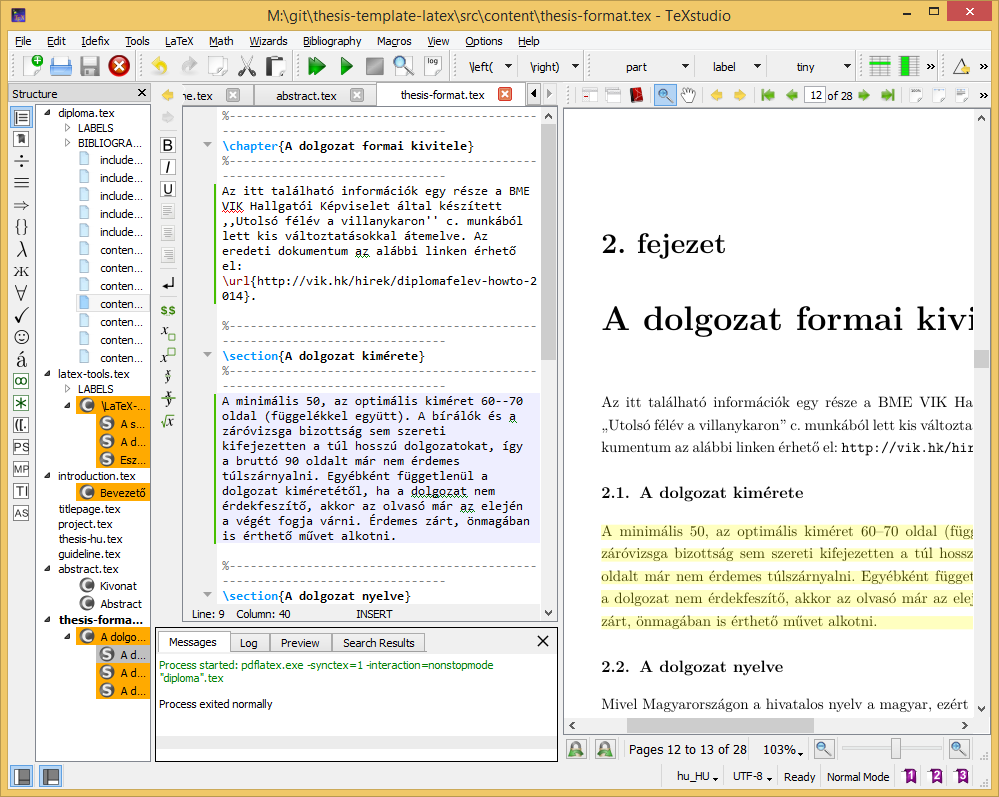
\includegraphics[width=150mm, keepaspectratio]{figures/TeXstudio.png}
\caption{A TeXstudio \LaTeX-szerkesztő.} 
\end{figure}

%----------------------------------------------------------------------------
\clearpage\section{Válasz az ,,Élet, a világmindenség, meg minden'' kérdésére}
%----------------------------------------------------------------------------
A Pitagorasz-tételből levezetve
\begin{align}
c^2=a^2+b^2=42.
\end{align}
A Faraday-indukciós törvényből levezetve
\begin{align}
\rot E=-\frac{dB}{dt}\hspace{1cm}\longrightarrow \hspace{1cm}
U_i=\oint\limits_\mathbf{L}{\mathbf{E}\mathbf{dl}}=-\frac{d}{dt}\int\limits_A{\mathbf{B}\mathbf{da}}=42.
\end{align}


%\label{page:last}
\end{document}
